%!TEX program = xelatex
%!TEX options=--shell-escape
\documentclass[12pt]{article}

%
\usepackage[scheme=plain]{ctex}
%
\usepackage{fontspec}
%
\usepackage[margin = 1in]{geometry}

%
\usepackage[dvipsnames]{xcolor}
\usepackage[many]{tcolorbox}

%
\usepackage{amsmath}
\usepackage{amssymb}
\usepackage{amsthm}
%
\usepackage{tensor}
%
\usepackage{slashed}
\usepackage{physics}
\usepackage{simpler-wick}

%
\usepackage[version=4]{mhchem}

%
\usepackage{mathtools}

%
\usepackage{bm}
\newcommand{\dbar}{\dif\hspace*{-0.18em}\bar{}\hspace*{0.2em}}
\DeclareMathAlphabet\mathbfcal{OMS}{cmsy}{b}{n}
%\usepackage{bbold}
\newcommand*{\dif}{\mathop{}\!\mathrm{d}}
\newcommand*{\euler}{\mathrm{e}}
\newcommand*{\imagi}{\mathrm{i}}

\renewcommand{\vec}[1]{\boldsymbol{\mathbf{#1}}}

\usepackage{caption}
\usepackage{multirow}
\usepackage{enumitem}

%
\usepackage{mathrsfs}
\usepackage{dsfont}

%
\usepackage{hyperref}
\hypersetup{
    colorlinks=true,
    linkcolor=violet,
    filecolor=blue,      
    urlcolor=blue,
    citecolor=cyan,
}

%
\usepackage{graphicx}
\usepackage{subfig}
%
\graphicspath{{figures/}{../figures/}}


%
\usepackage{indentfirst}
%
\setlength{\parindent}{2em}
\linespread{1.25}

% 
% \setmainfont{Times New Roman}

\title{Note}
\author{Feng-Yang Hsieh}
\date{}

\begin{document}
\maketitle

\section{CWoLa}% (fold)
\label{sec:cwola}
	The Classification Without Labels (CWoLa) is a weakly supervised learning method. The CWoLa approach trains a model to discriminate the mixed samples, which are mixtures of the original signal and background samples. The optimal classifier in the CWoLa approach is also the optimal classifier in the traditional fully supervised case where all label information is available. This section utilizes the CWoLa approach to train classifiers on di-Higgs samples.

	\subsection{Sample}% (fold)
	\label{sub:sample}
		This exercise's signal corresponds to the resonant Higgs boson pairs production in the four-$b$ quarks channel. These Higgs boson pairs are produced via gluon-gluon fusion in the two Higgs doublet model (2HDM). The Higgs boson $h$ ($m_h = \text{125 GeV}$) pair is produced by the heavy CP-even scalar $H$ with mass $m_H$ ranging from $\text{300 GeV}$ to $\text{1200 GeV}$. The background consists of QCD multi-jet events.

		The CWoLa training samples $M_1$ and $M_2$ are the mixtures of the signal and background samples. The probability distribution of the mixed sample is a combination of the signal $p_s(x)$ and background $p_B(x)$ distributions:
		\begin{equation}
			\begin{aligned}
				p_{M_1}(x) &=  f_1 p_S(x) + (1-f_1) p_B(x) \\
				p_{M_2}(x) &=  f_2 p_S(x) + (1-f_2) p_B(x)
			\end{aligned}
		\end{equation}
		where $f_1, f_2$ are the signal fractions, and $x$ represents the observables used for the classification task.

		DNN and SPANet network architectures are considered in this exercise. For DNN, the input features are summarised in Table \ref{tab:DNN_variables}, consisting of 16 variables. For SPANet, the input features are a list of final jets, each represented by their 4-momentum $(p_\text{T}, \eta,\phi, M)$ and a boolean $b$-tag.
		\begin{table}[htpb]
			\centering
			\caption{Input variables used to train the dense neural network.}
			\label{tab:DNN_variables}
			\begin{tabular}{l|c|c}
				Reconstructed objects       & Variables used for training   & \# \\ \hline
				Higgs candidate             & $(p_\text{T}, \eta, \phi, m)$ & 8  \\
				Subjets                     & $\Delta R(j_1,j_2)$                    & 2  \\
				b-tagging                   & Boolean for $j_i \in h_{1,2}^{\text{cand}}$       & 4  \\
				Di-Higgs system             & $p_\text{T}^{hh}, m_{hh}$        & 2 
			\end{tabular}		
		\end{table}

	% subsection sample (end)
	\subsection{Result}% (fold)
	\label{sub:result}
		The CWoLa training utilizes samples with different signal fractions $f_1,f_2$ to train the classifiers. The results of CWoLa training are shown in Figure~\ref{fig:CWoLa_training_result} with different signal fractions. When $f_1$ is far from $0.5$, the results tend to approach those of the fully supervised case.
		\begin{figure}[htpb]
			\centering
			\subfloat[DNN]{
				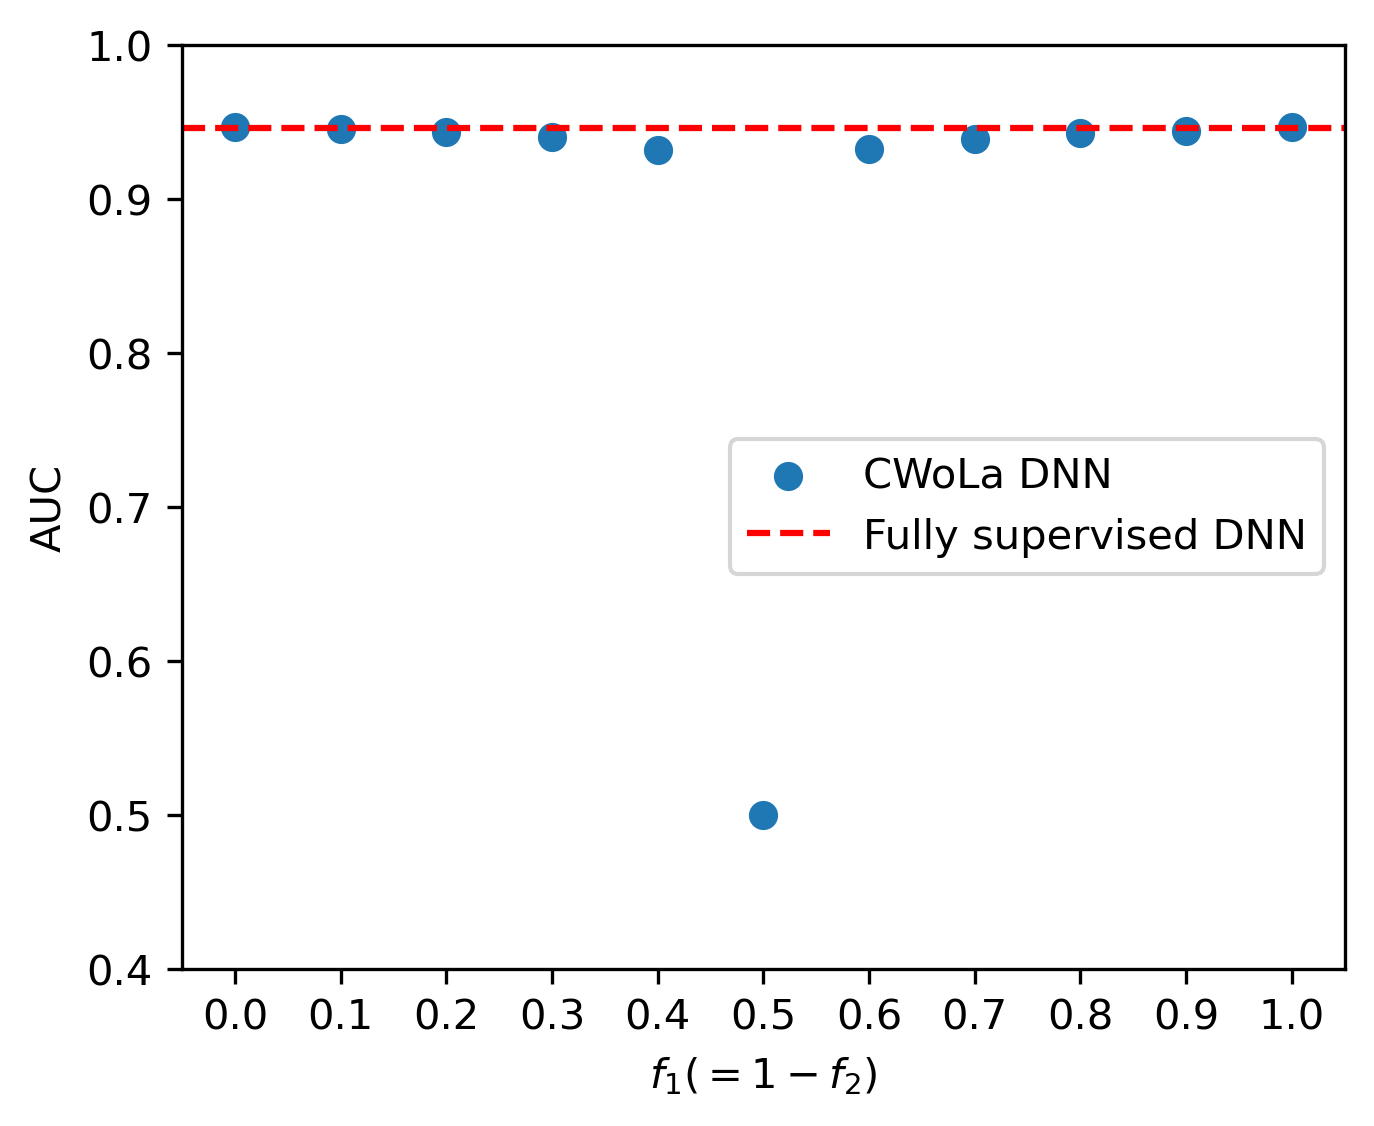
\includegraphics[width=0.45\textwidth]{CWoLa_DNN.png}
			}
			\subfloat[SPANet]{
				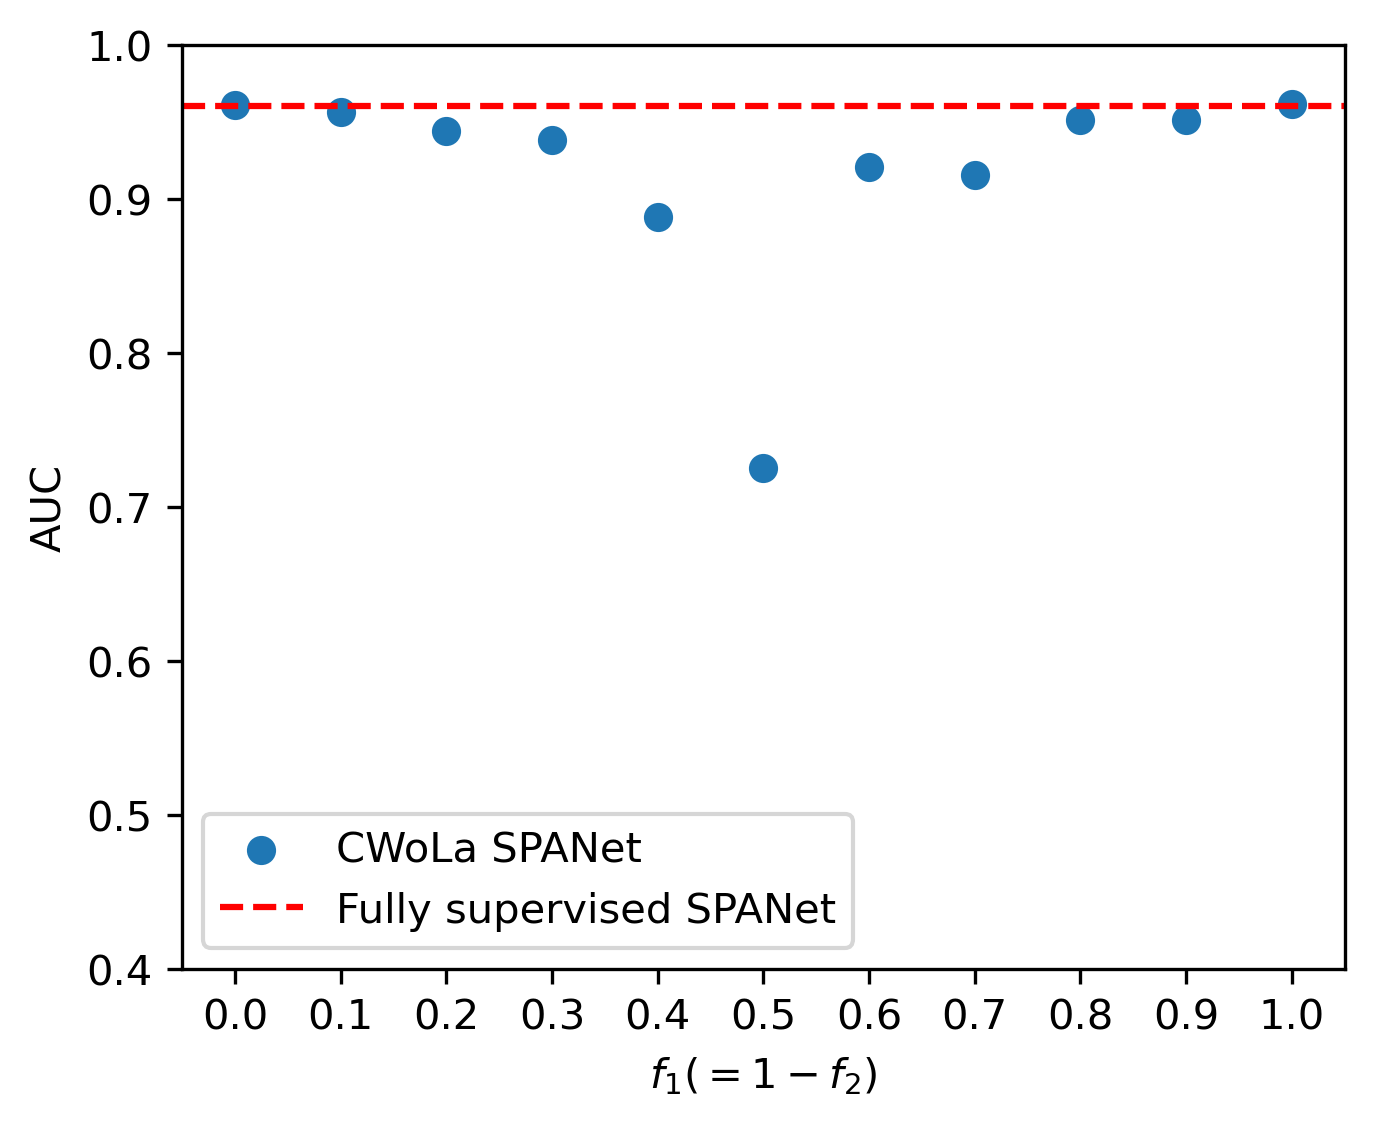
\includegraphics[width=0.45\textwidth]{CWoLa_SPANet.png}
			}
			\caption{The AUC of CWoLa training as a function of the signal fraction $f_1$. For simplicity, we set signal fraction $f_2$ equal to $1 - f_1$. The horizontal dashed line indicates the fully-supervised AUC.}
			\label{fig:CWoLa_training_result}
		\end{figure}

		When $f_1 = 0.5$ the mixed sample $M_1$ and $M_2$ have identical distributions, so the classifier can not learn anything in this case. In the case of DNN, the AUC is $0.5$, as expected. However, for SPANet, the AUC is more than $0.7$.

		This is because SPANet is trained on both pairing and classification tasks simultaneously. The pairing part introduces some asymmetries between signal and background samples, leading to the AUC that deviates from $0.5$.

		To investigate the effect of the pairing task on SPANet's performance, the weight of the pairing component is set to zero, meaning that SPANet focuses solely on the classification task. Figure~\ref{fig:CWoLa_SPANet_without_pairing} shows the SPANet training results without pairing task. As expected, the AUC is close to $0.5$ when $f_1 = 0.5$. 
		\begin{figure}[htpb]
			\centering
			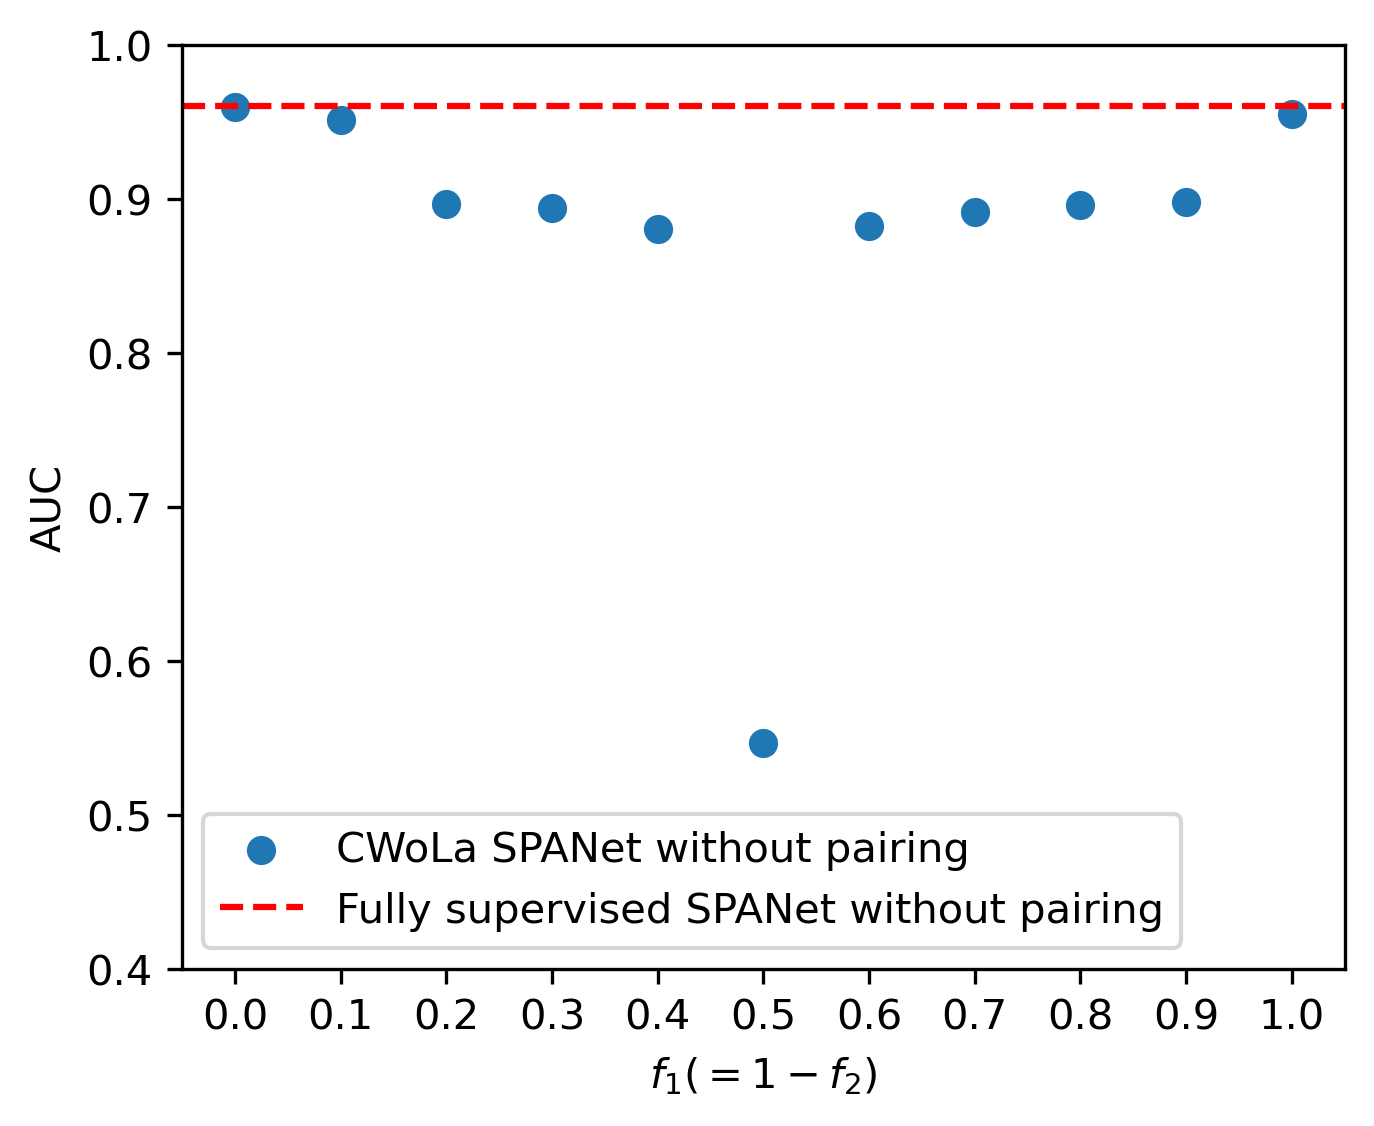
\includegraphics[width=0.65\textwidth]{CWoLa_SPANet_no_pair.png}
			\caption{The AUC of CWoLa SPANet training as a function of the signal fraction $f_1$. For simplicity, we set signal fraction $f_2$ equal to $1 - f_1$. Here, SPANet is trained on the classification task only.}
			\label{fig:CWoLa_SPANet_without_pairing}
		\end{figure}	
	% subsection result (end)	
% section cwola (end)

\section{CWoLa hunting}% (fold)
\label{sec:cwola_hunting}
	The CWoLa hunting approach considers a variable $m_{\text{res}}$. For background, the $m_{\text{res}}$ distribution is smooth while signal $m_{\text{res}}$ distribution is expected to be localized near some $m_0$. Consequently, this variable could be used to create two mixed samples. Additional features that are uncorrelated with $m_{\text{res}}$ can be used for training a classifier.
	\subsection{Sample}% (fold)
	\label{sub:sample_cwola_hunting}
		The signal is the resonant Higgs boson pairs production in the four-$b$ quarks channel. In this section, the Higgs boson pair is produced by the heavy CP-even scalar $H$ with mass $m_H = \text{500 GeV}$ or $m_H = \text{1000 GeV}$. The background consists of QCD multi-jet events. The basic requirement is the ``four-tag cut,'' which requires at least four $b$-tagged $R = 0.4$ anti-$k_t$ jets with $p_\text{T} > \text{40 GeV}$ and $\abs{\eta} < 2.5$. Only the events passing the four-tag cut are used in the following analysis.
		
		The CWoLa hunting approach utilizes the signal and sideband regions to create the mixed training sample. The di-Higgs system's total invariant mass $m_{hh}$ is utilized to determine the signal and sideband region. This quantity is computed from the four $b$-jets with the highest transverse momentum. Figure~\ref{fig:mhh_distribution} presents the $m_{hh}$ distribution of signal and background samples. Table~\ref{tab:signal_sideband_range} summarizes the signal and sideband regions. These signal and sideband regions are chosen such that the corresponding cross-sections are closed.
		\begin{figure}[htpb]
			\centering
			\subfloat[$m_H = \text{500 GeV}$]{
				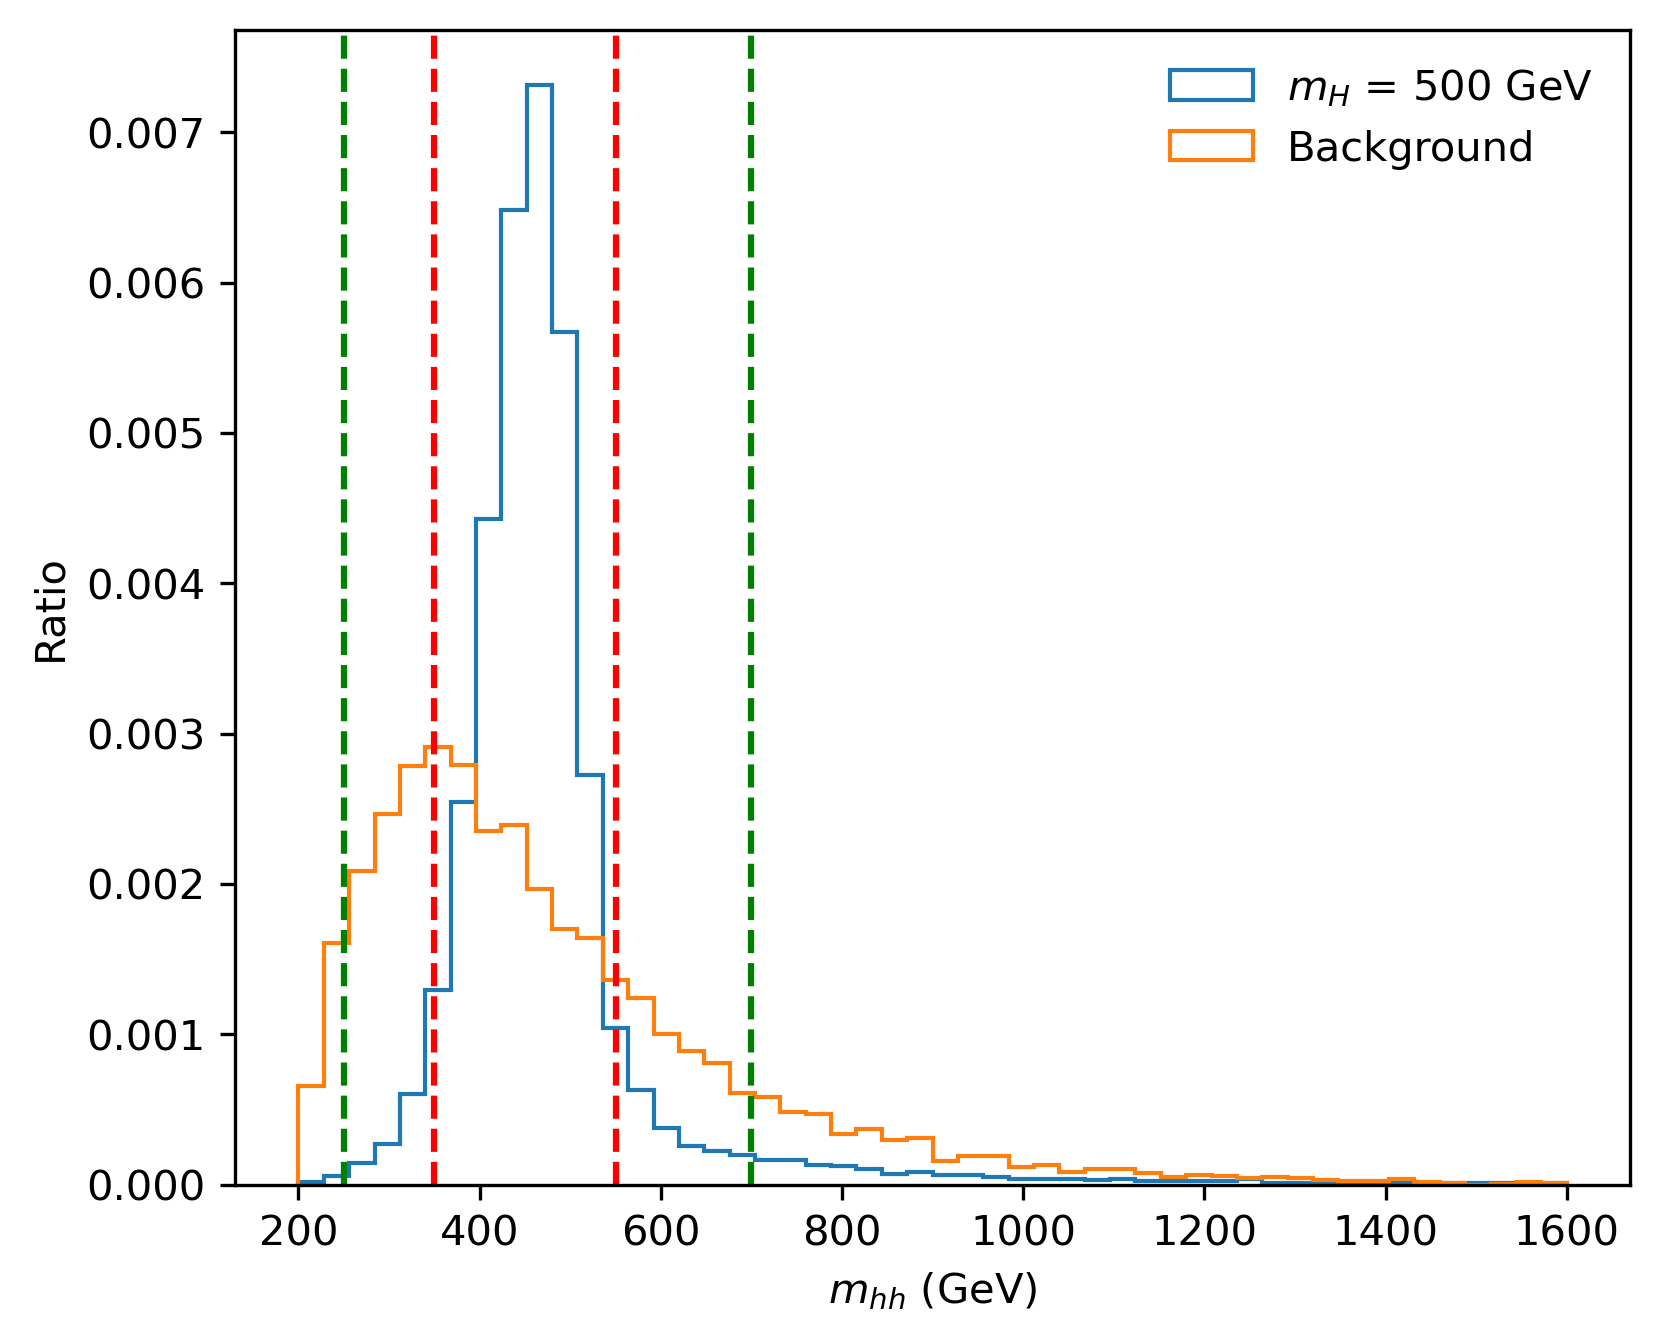
\includegraphics[width=0.45\textwidth]{mhh_distribution-500GeV.png}
			}
			\subfloat[$m_H = \text{1000 GeV}$]{
				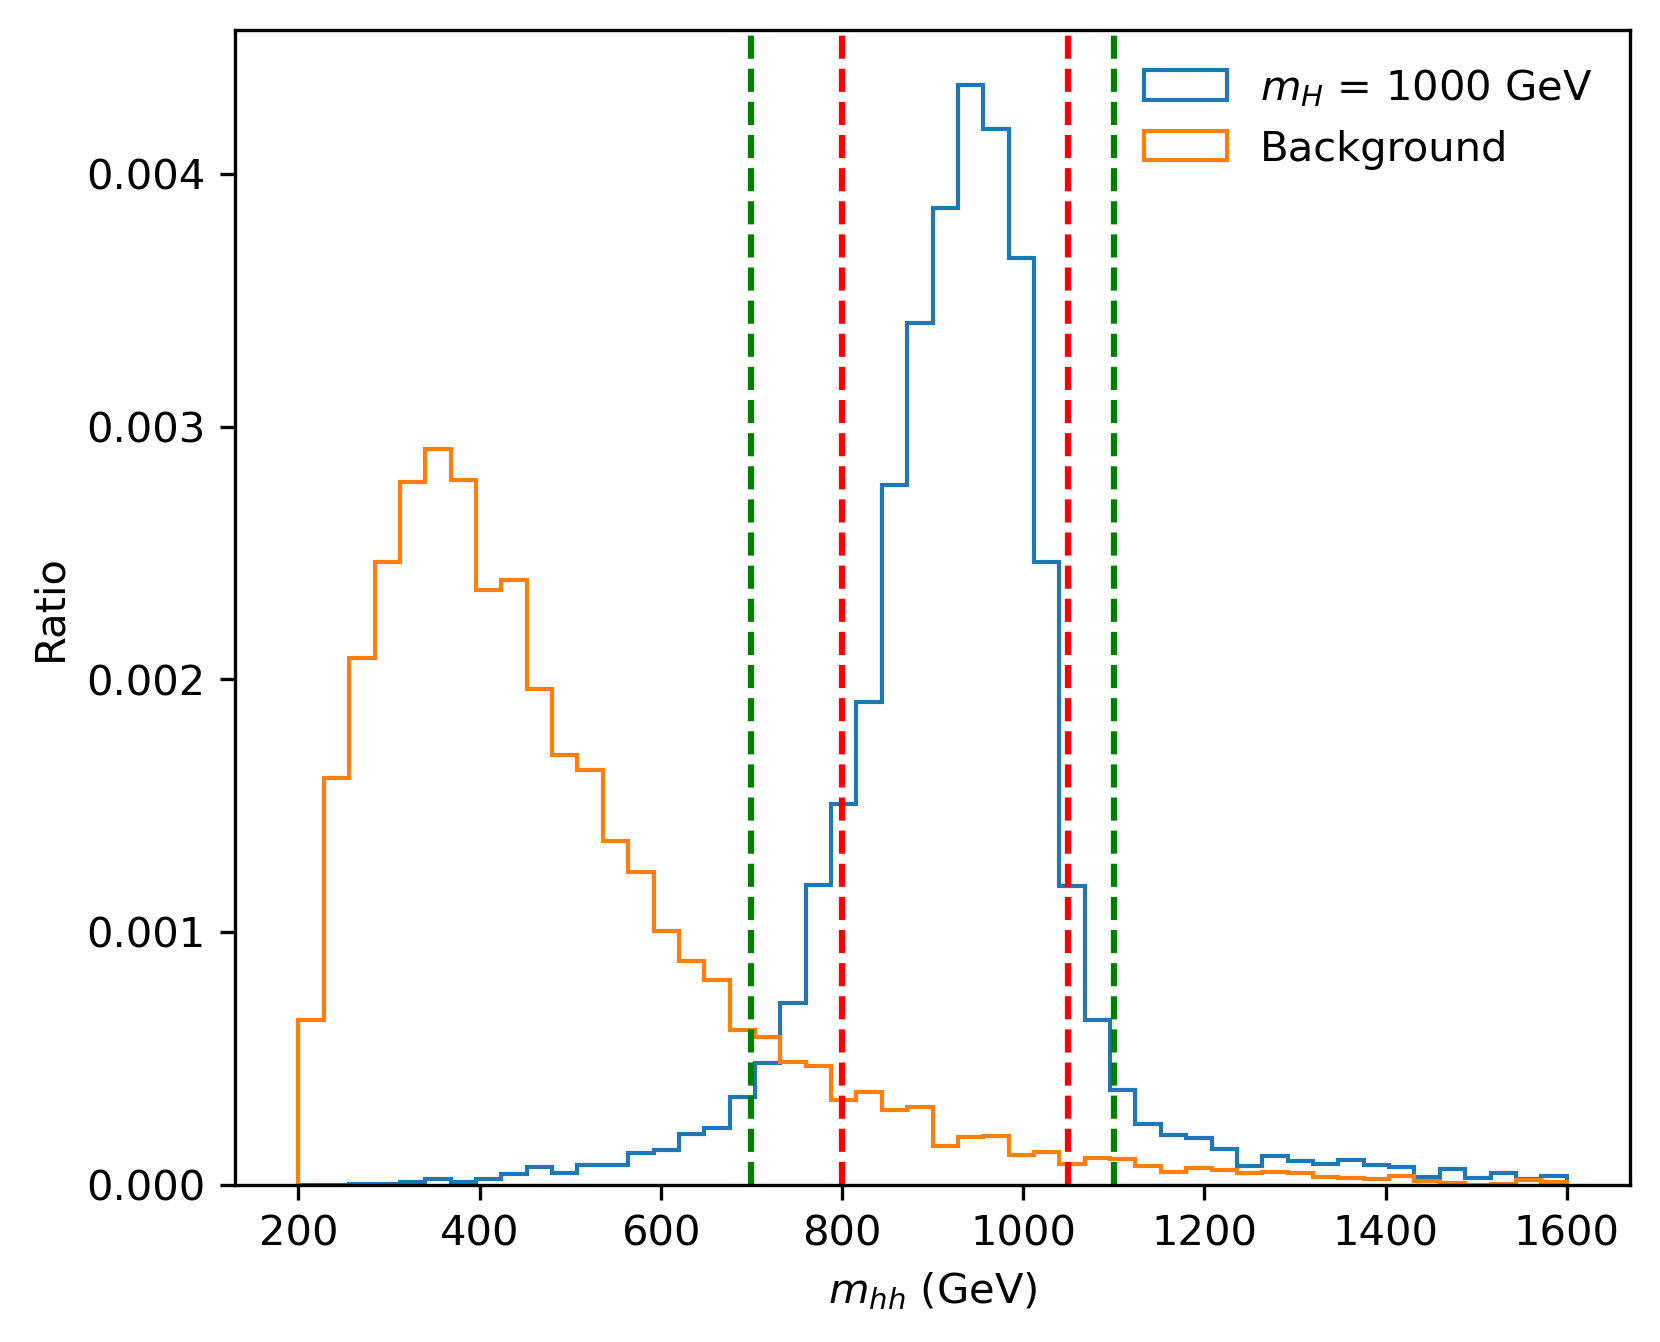
\includegraphics[width=0.45\textwidth]{mhh_distribution-1000GeV.png}
			}
			\caption{The totoal invriant mass $m_{hh}$ distribution of signal and background samples. The signal region is between the red dashed lines. The sideband region is between the green dashed lines and excludes the signal region.}
			\label{fig:mhh_distribution}
		\end{figure}

		\begin{table}[htpb]
			\centering
			\caption{The signal and sideband regions with different resonant samples. The unit is GeV.}
			\label{tab:signal_sideband_range}
			\begin{tabular}{r|cc}
				$m_H$ & Signal       & Sideband                      \\ \hline
				500   & $[350, 550]$ & $[250, 350]\cup [550, 700]$   \\
				1000  & $[800,1050]$ & $[700, 800]\cup [1050, 1100]$
			\end{tabular}
		\end{table}
		Table~\ref{tab:diHiggs_cutflow_table} is the cutflow table of the selection cuts. The number of events used in mixed training samples could be computed from these cross-sections. The training sample size is presented in Table~\ref{tab:training_sample_size_cwola_hunting}.
		\begin{table}[htpb]
			\centering
			\caption{The cross sections for the di-Higgs signal and background processes at different selection cuts.}
			\label{tab:diHiggs_cutflow_table}
			\begin{tabular}{c|l|cc|c|c}
									  &                 & \multicolumn{2}{c|}{Cross section (fb)} &          & $\mathcal{L} = 139 \text{ fb}^{-1}$ \\
				$m_H$ (GeV)           &                 & Signal           & Background           & $S / B$  & $S/\sqrt{B}$                        \\ \hline 
				\multirow{3}{*}{500}  & Four tag        & 3.64             & 6.03e+03             & 6.03e-04 & 0.553                               \\ \cline{2-6} 
									  & Signal region   & 3.13             & 2.57e+03             & 1.22e-03 & 0.727                               \\
									  & Sideband region & 0.35             & 2.36e+03             & 1.50e-04 & 0.086                               \\ \hline \hline
				\multirow{3}{*}{1000} & Four tag        & 0.081            & 6.03e+03             & 1.34e-05 & 0.0123                              \\ \cline{2-6} 
									  & Signal region   & 0.063            & 3.32e+02             & 1.90e-04 & 0.0408                              \\
									  & Sideband region & 0.010            & 3.19e+02             & 3.03e-05 & 0.0064                             
			\end{tabular}
		\end{table}
		
		\begin{table}[htpb]
			\centering
			\caption{The training sample size for the mixed sample. The luminosity is $\mathcal{L} = 78 \text{ fb}^{-1}$ because the generated samples are not enough for now.}
			\label{tab:training_sample_size_cwola_hunting}
			\begin{tabular}{c|c|cc}
									  &              & \multicolumn{2}{c}{True label} \\
				$m_H$ (GeV)           & Mixed sample & Signal       & Background      \\ \hline
				\multirow{2}{*}{500}  & $M_1$        & 244          & 200k            \\
									  & $M_2$        & 28           & 184k            \\ \hline
				\multirow{2}{*}{1000} & $M_1$        & 5            & 26k             \\
									  & $M_2$        & 1            & 25k            
			\end{tabular}
		\end{table}

		Consider the DNN CWoLa classifier. The Higgs candidates are reconstructed by the $\text{min-}\Delta R$ pairing method. In the $\text{min-}\Delta R$ method, the four $b$-tagged jets with the highest $p_{\text{T}}$ are used to form the two Higgs boson candidates. The $\text{min-}\Delta R$ method selects the pairing configuration in which the higher-$p_{\text{T}}$ jet pair has the smallest $\Delta R$ separation. The input features are similar to the previous case (Table~\ref{tab:DNN_variables}), but the $b$-tagging information and the di-Higgs system's total invariant mass are excluded. For $\text{min-}\Delta R$ pairing, it only uses the $b$-tagged jets. Total invariant mass is already used to determine the signal and sideband region.

	% subsection sample_cwola_hunting (end)
	\subsection{Training results}% (fold)
	\label{sub:training_results}
		Table \ref{tab:cwola_hunting_DNN_results} presents the DNN classification training results. These numbers are evaluated from the pure samples, which consist of 5k signal events and 5k background events. The training datasets with and without signal events have similar results. This suggests that the DNN fails to distinguish the signal and background samples but learns the difference between the signal and sideband region. Moreover, the results also imply the input features may correlate to the total invariant mass of the di-Higgs system.
		\begin{table}[htpb]
			\centering
			\caption{The CWoLa DNN training results. ACC is the best accuracy and AUC is the area under the ROC curve. The average and standard deviation of 10 training are presented.}
			\label{tab:cwola_hunting_DNN_results}
			\begin{tabular}{c|c|cc}
				$m_H$ (GeV)           &             & ACC               & AUC               \\ \hline
				\multirow{2}{*}{500}  & With signal & $0.708 \pm 0.002$ & $0.770 \pm 0.007$ \\
									  & No signal   & $0.705 \pm 0.003$ & $0.769 \pm 0.009$ \\ \hline
				\multirow{2}{*}{1000} & With signal & $0.868 \pm 0.024$ & $0.925 \pm 0.023$ \\
									  & No signal   & $0.850 \pm 0.033$ & $0.909 \pm 0.026$
			\end{tabular}
		\end{table}

		Figure~\ref{fig:signal_score_distribution} shows the signal score distributions. Even though the signal scores are very different for signal and background distributions, the difference probably stems from the $m_{hh}$ distribution.
	 	\begin{figure}[htpb]
			\centering
			\subfloat[$m_H = \text{500 GeV}$]{
				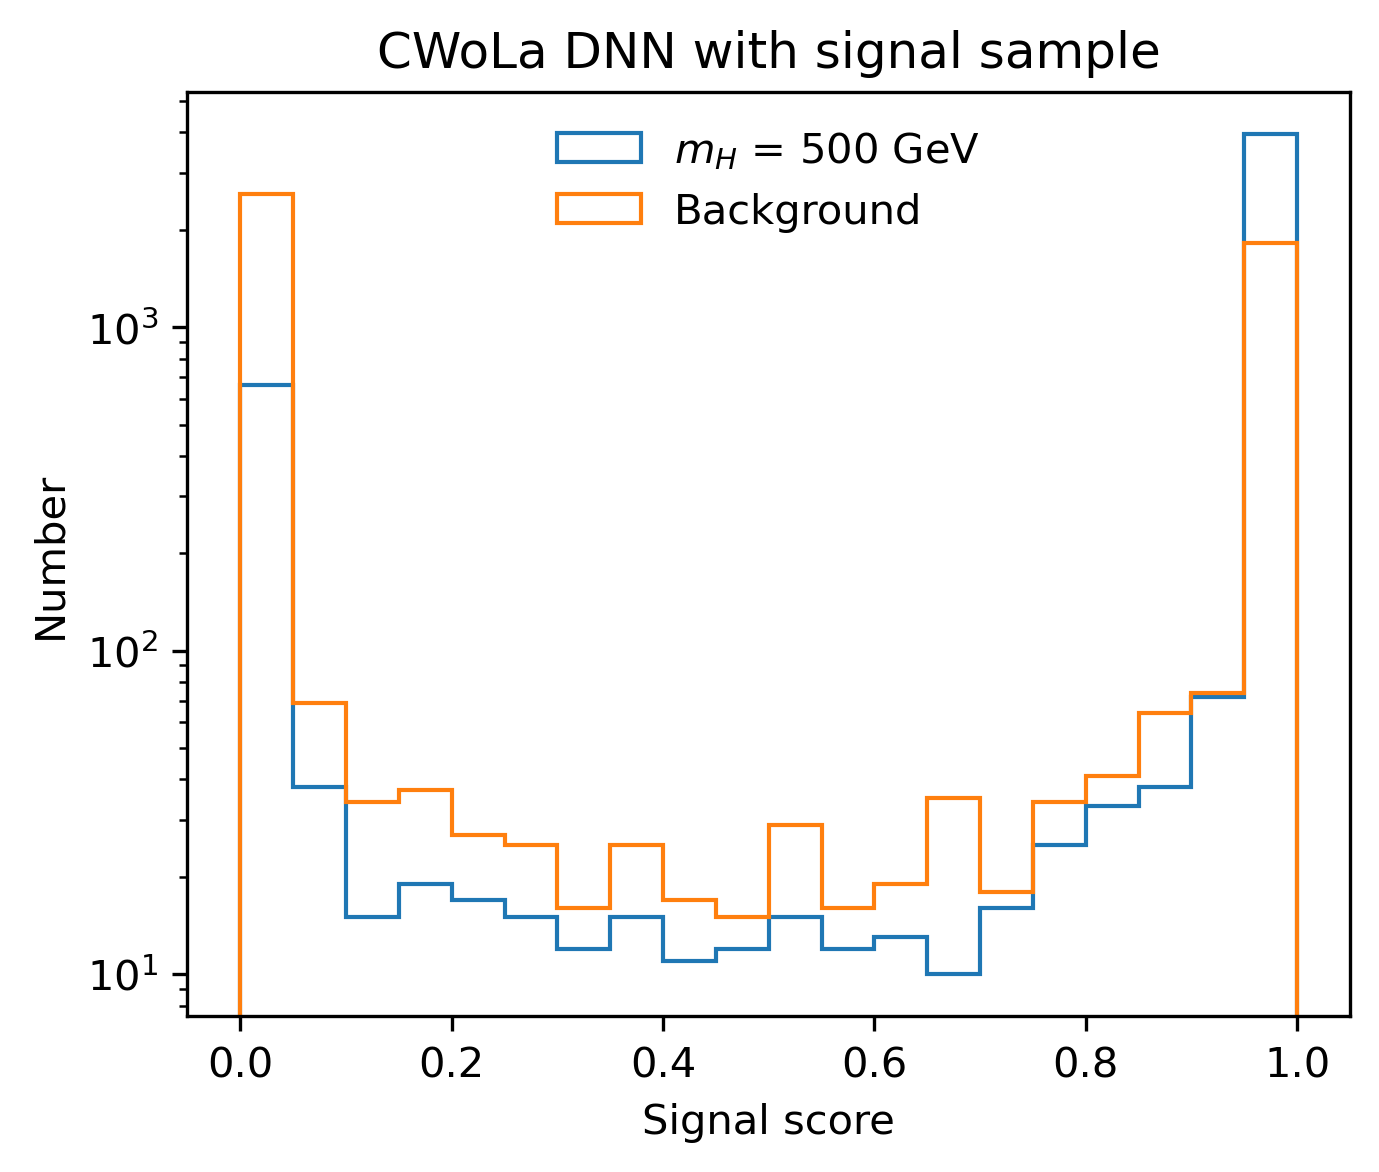
\includegraphics[width=0.45\textwidth]{DNN_w_sig_signal_score_distribution-500GeV.png}
				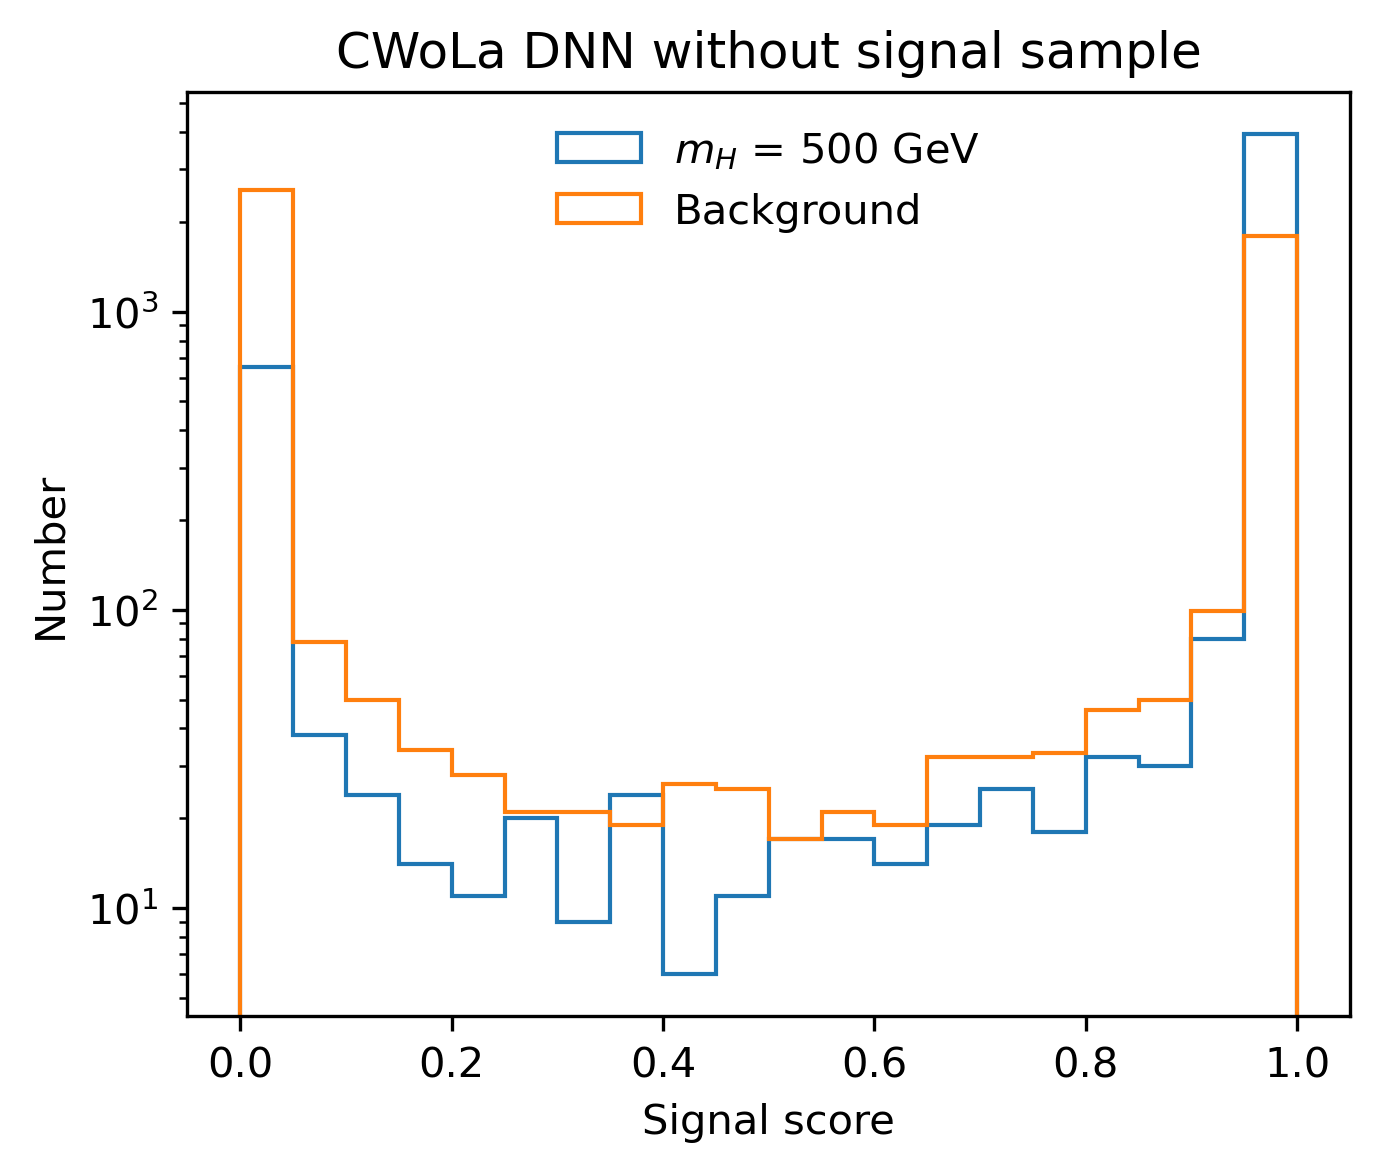
\includegraphics[width=0.45\textwidth]{DNN_wo_sig_signal_score_distribution-500GeV.png}
			}
			\\
			\subfloat[$m_H = \text{1000 GeV}$]{
				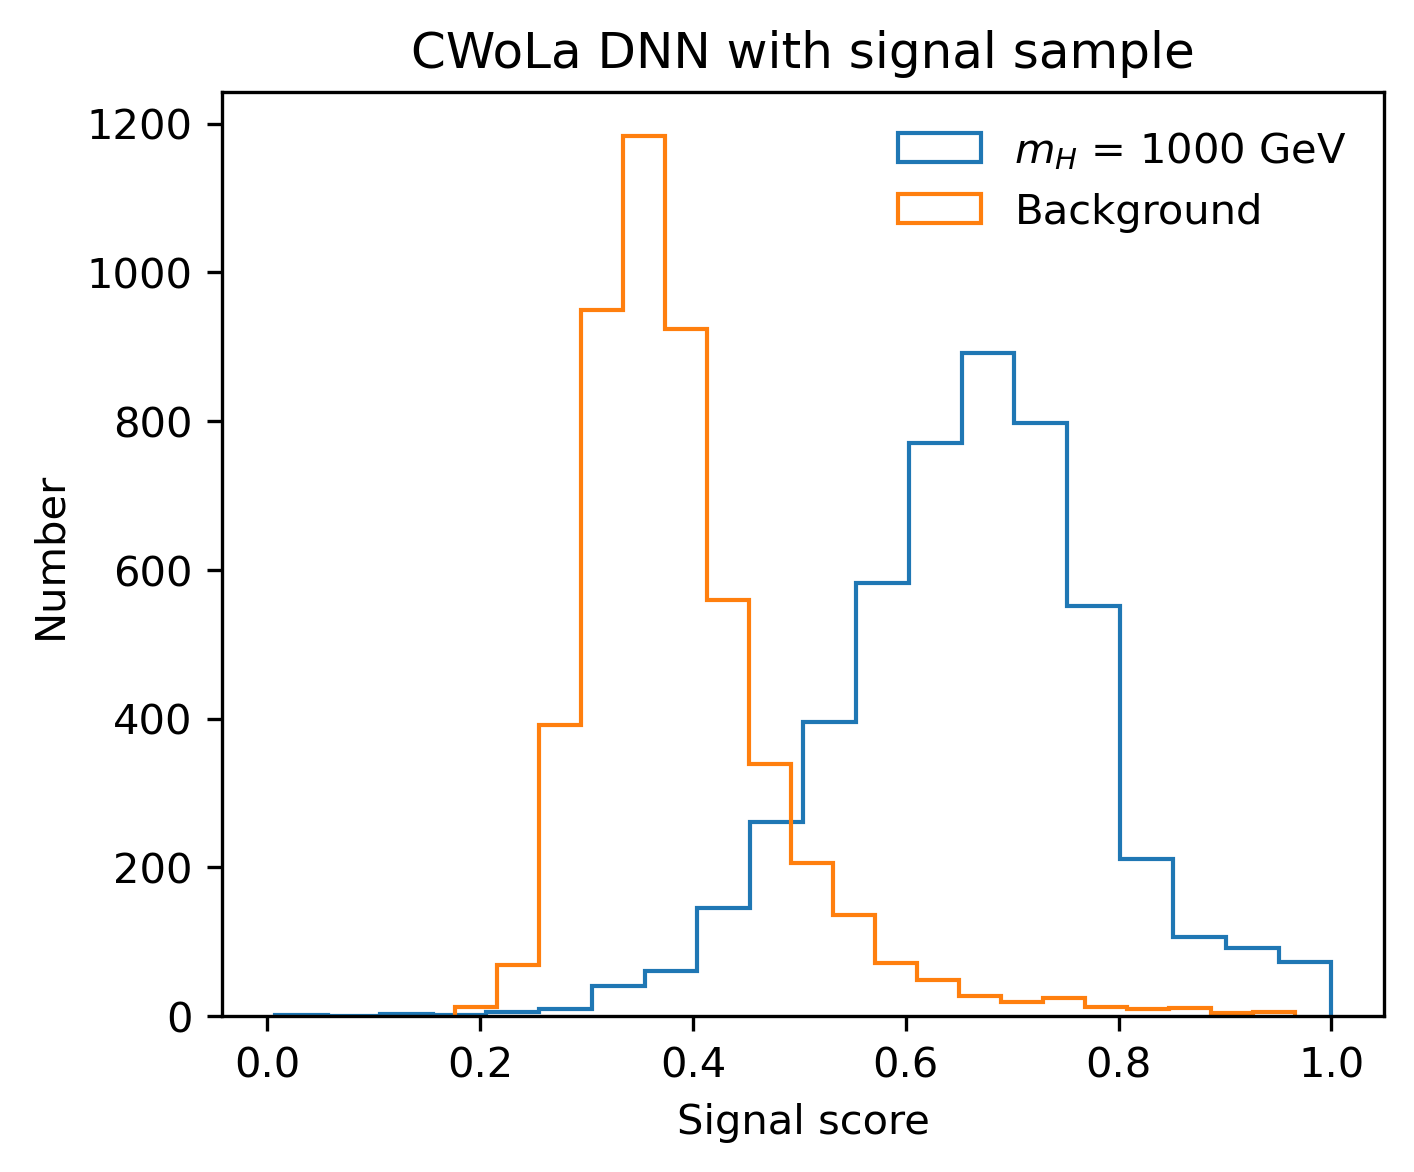
\includegraphics[width=0.45\textwidth]{DNN_w_sig_signal_score_distribution-1000GeV.png}
				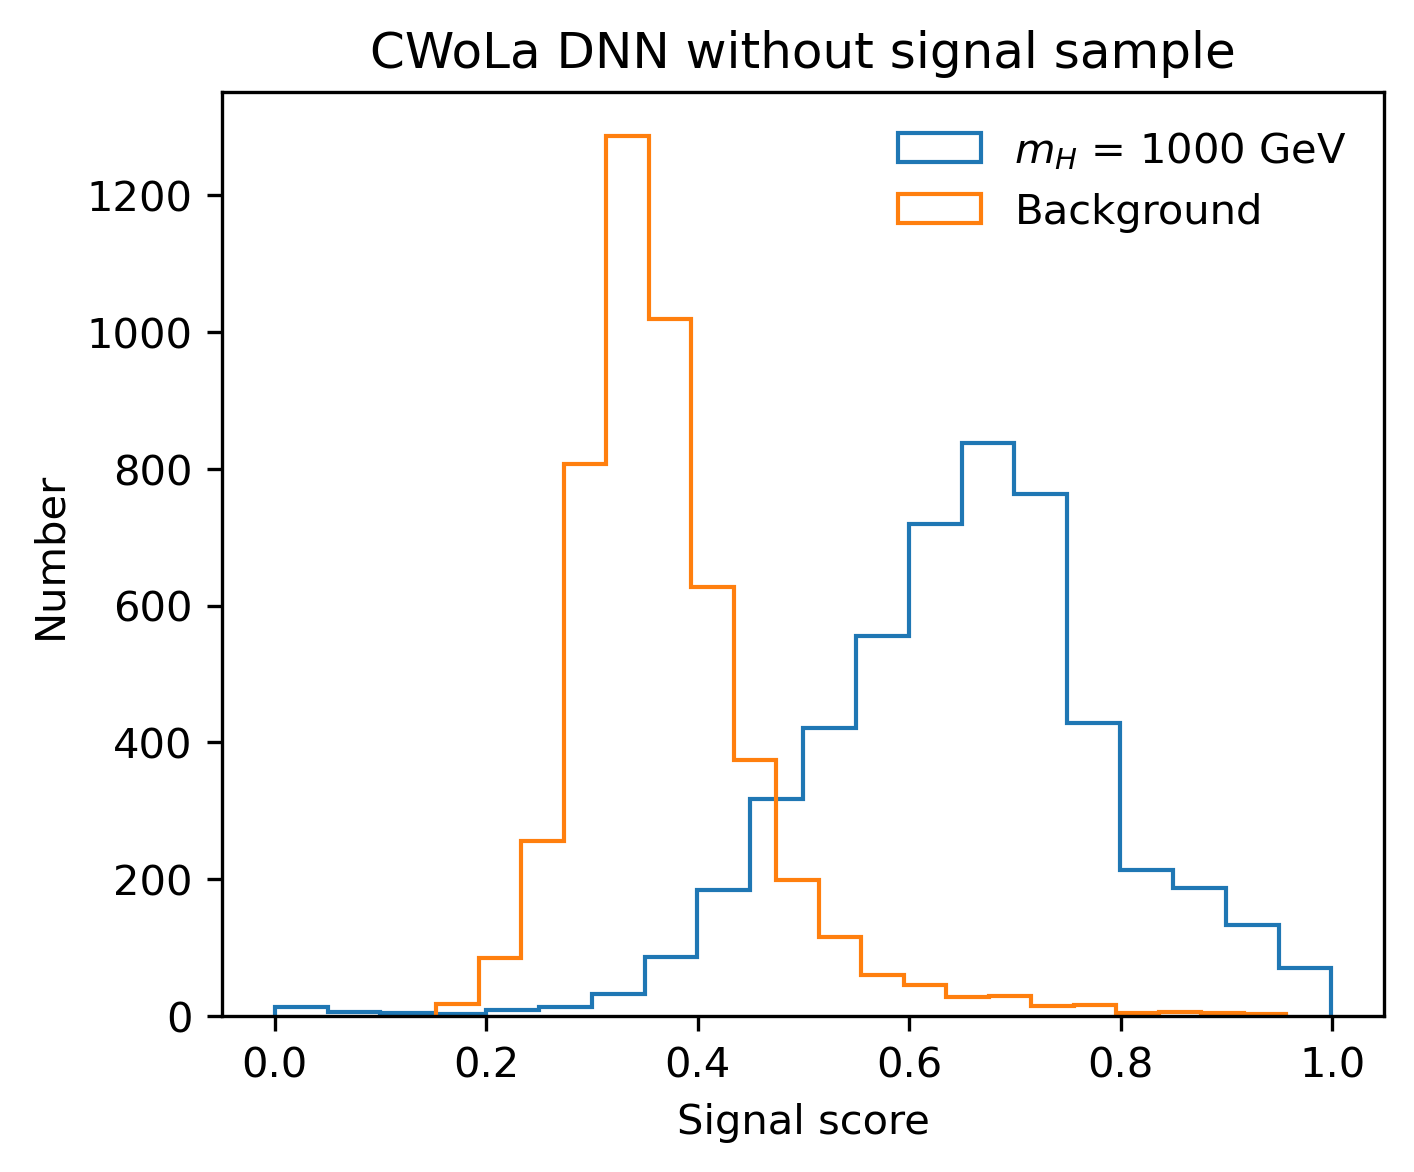
\includegraphics[width=0.45\textwidth]{DNN_wo_sig_signal_score_distribution-1000GeV.png}
			}
			\caption{The signal score distributions. We apply the CWoLa DNN on pure samples to obtain the signal score distributions.}
			\label{fig:signal_score_distribution}
		\end{figure}

		There are two issues:
		\begin{itemize}
			\item The input features might correlated to the observables used to determine the signal and sideband region. We need to construct other independent input variables.
			\item The signal fraction is too low. It is hard to learn something about signal events. 
		\end{itemize}
	% subsection training_results (end)
	\subsection{Correlation matrix}% (fold)
	\label{sub:correlation_matrix}
		The results in Section~\ref{sub:training_results} imply that the di-Higgs system's total invariant mass is not independent of other input features. To find the variables that are highly dependent on the total invariant mass, the correlation coefficients are computed among these variables. Figure~\ref{fig:correlation_coefficient_500GeV} and \ref{fig:correlation_coefficient_1000GeV} are correlation coefficients on the $\text{500 GeV}$ and $\text{1000 GeV}$ cases, respectively. 

		\begin{figure}[htpb]
			\centering
			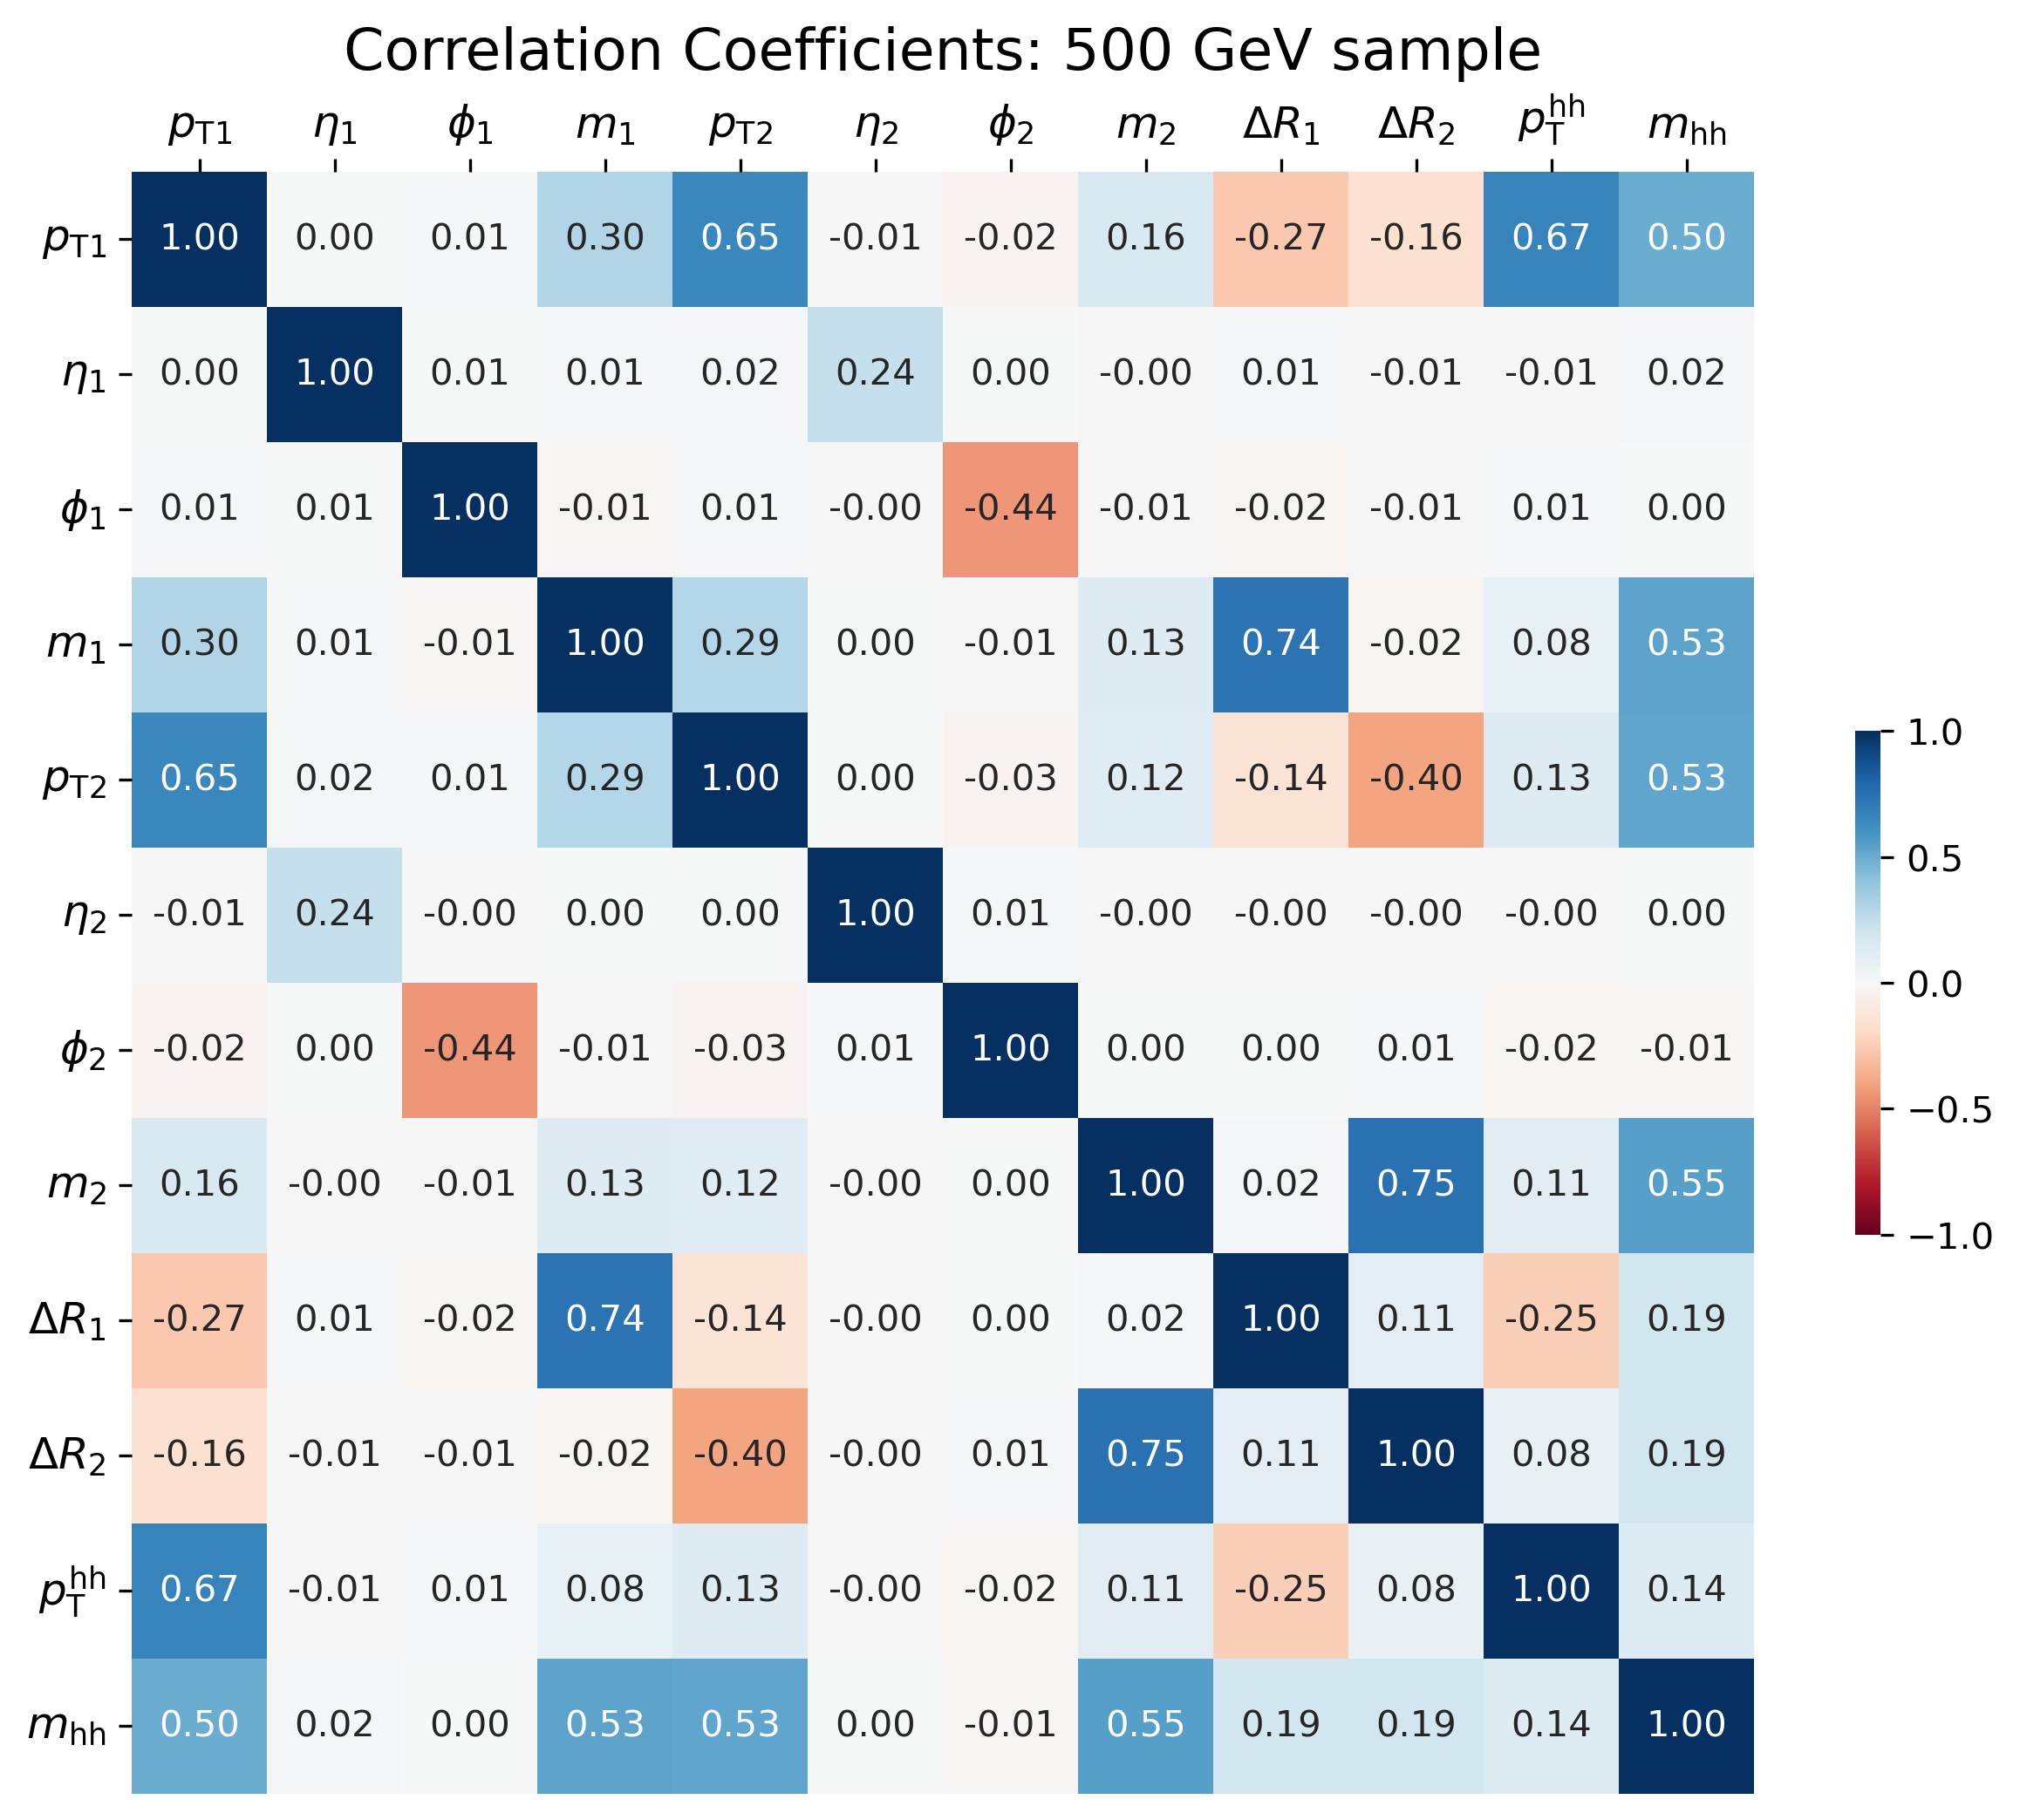
\includegraphics[width=0.9\textwidth]{correlation_coefficients-500GeV.png}
			\caption{The correlation coefficients among different variables, which are computed from $\text{500 GeV}$ testing sample, which consists of 5k signal and 5k background.}
			\label{fig:correlation_coefficient_500GeV}
		\end{figure}
		
		\begin{figure}[htpb]
			\centering
			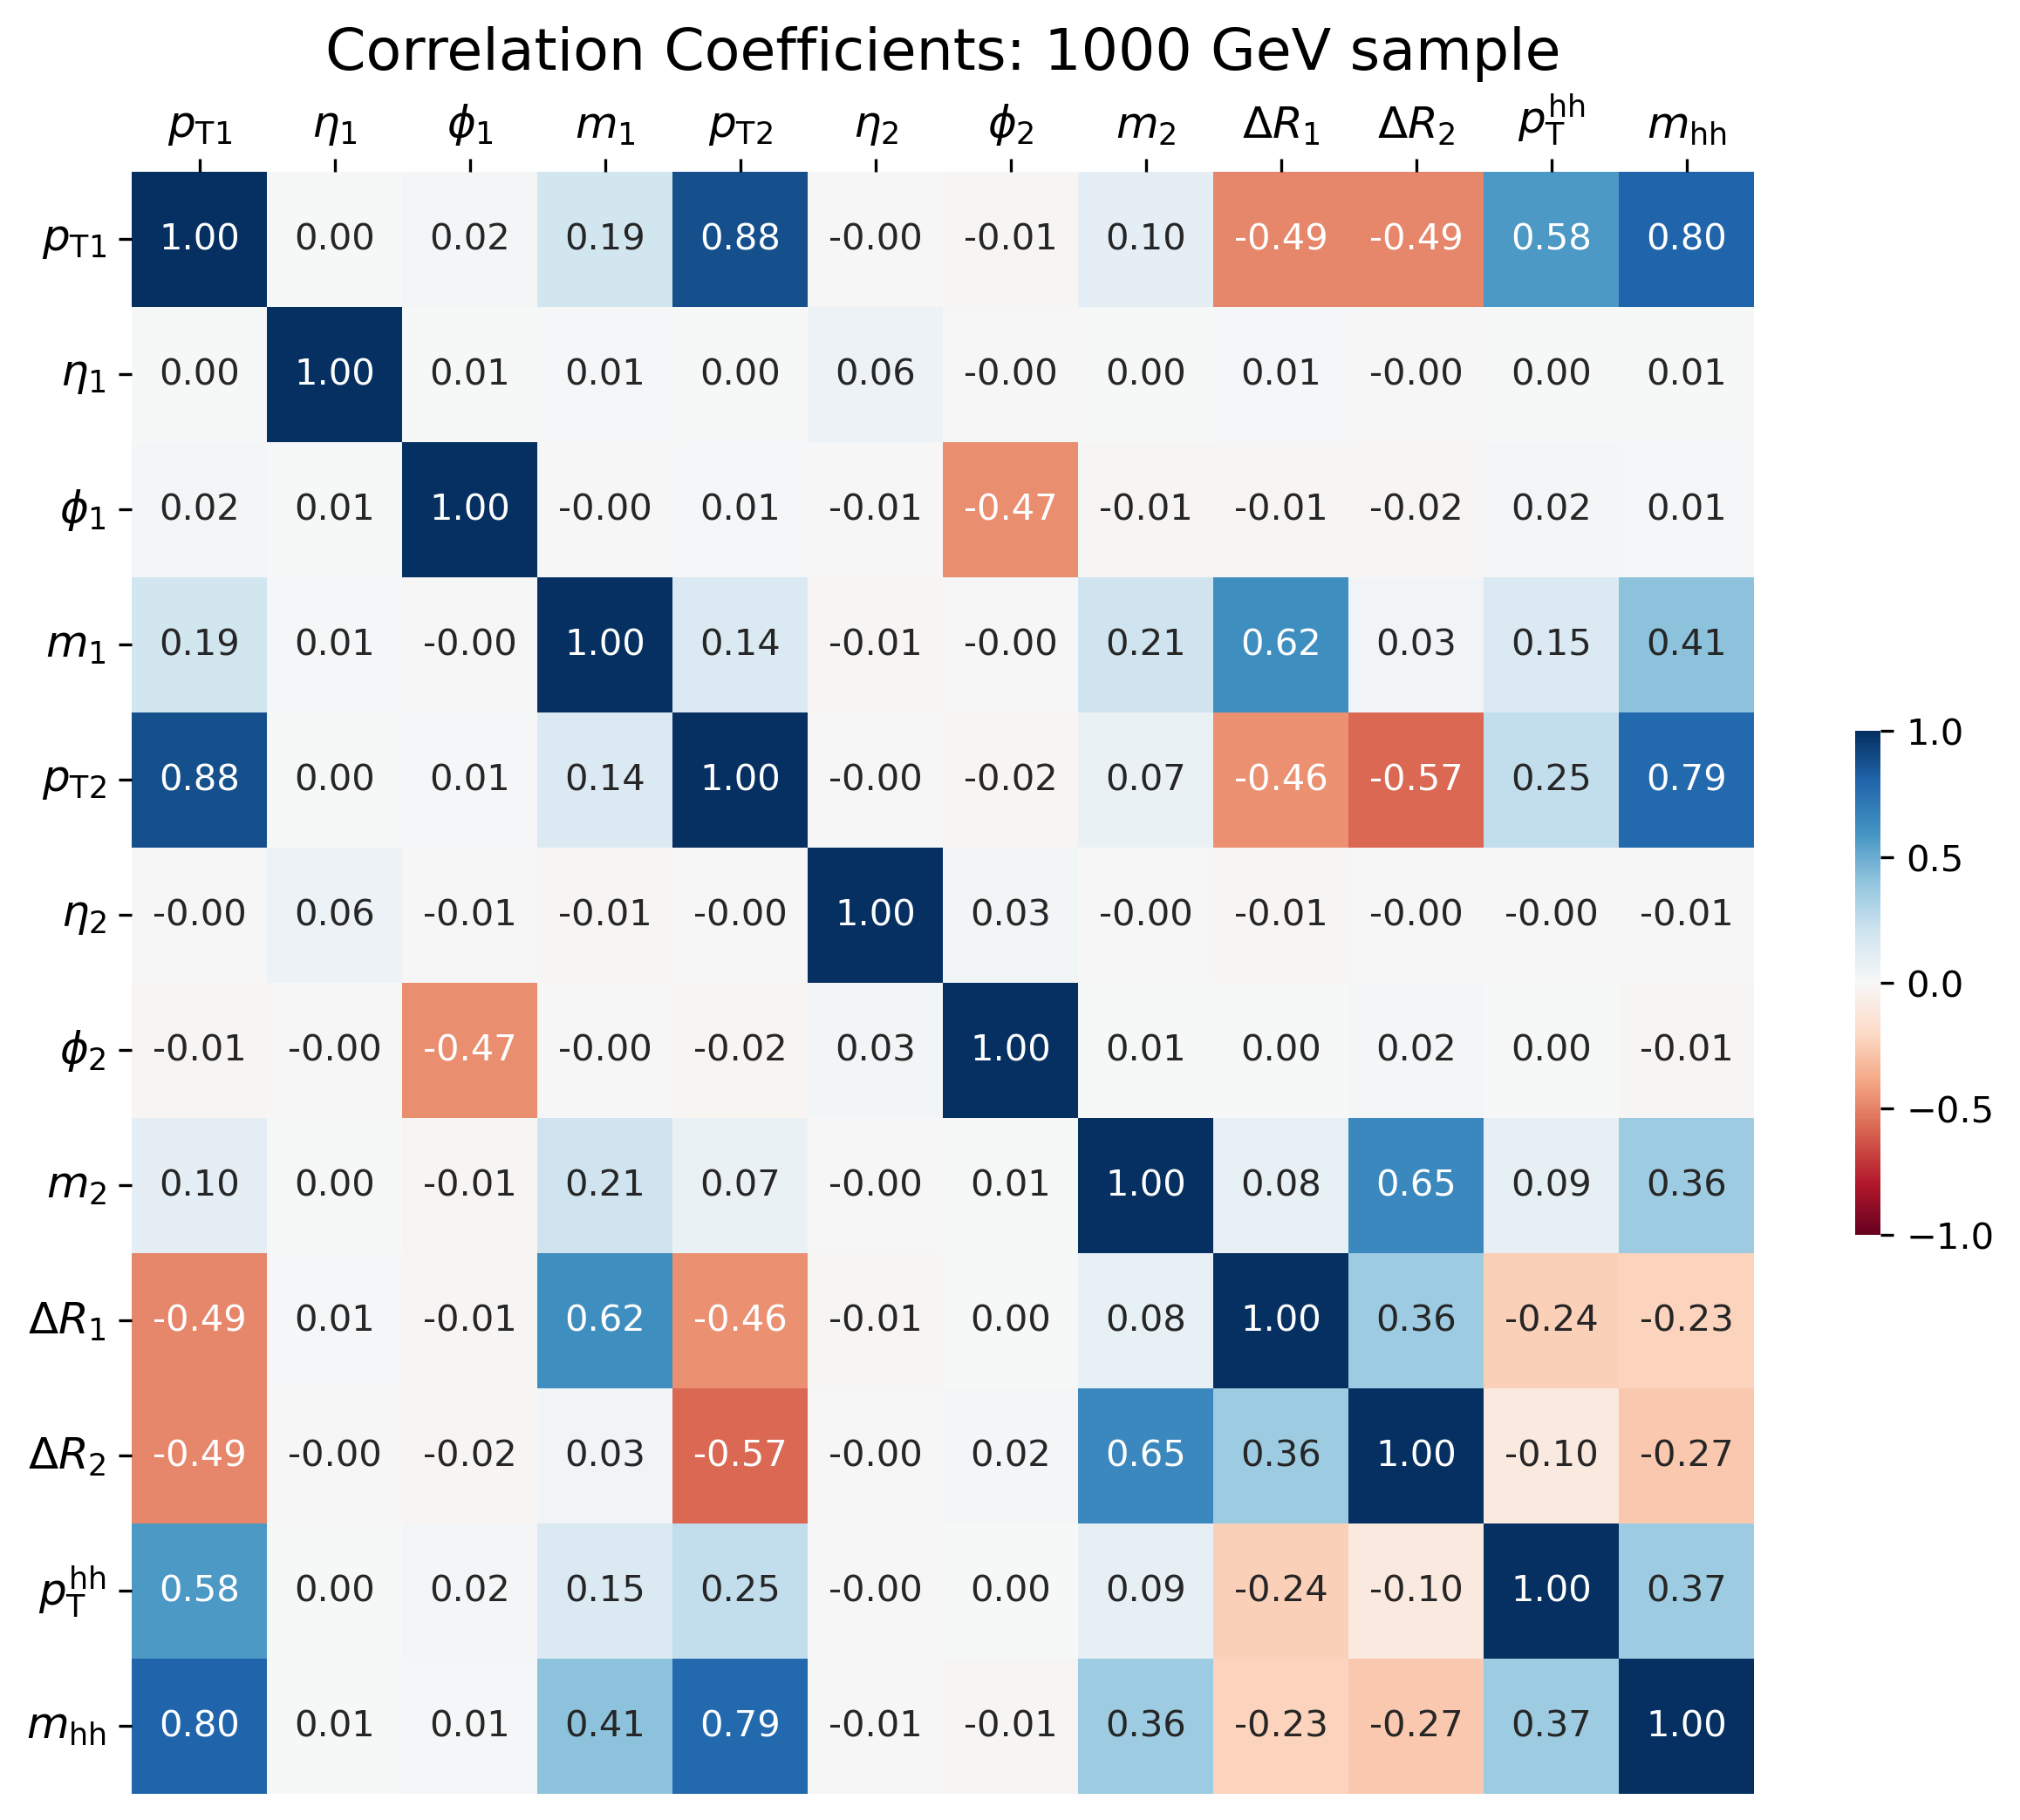
\includegraphics[width=0.9\textwidth]{correlation_coefficients-1000GeV.png}
			\caption{The correlation coefficients among different variables, which are computed from $\text{1000 GeV}$ testing sample, which consists of 5k signal and 5k background.}
			\label{fig:correlation_coefficient_1000GeV}
		\end{figure}

		The results show that the transverse momentum $p_\text{T}$ and the invariant mass $m$ of Higgs candidates are highly correlated to the total invariant mass. Figure~\ref{fig:pt1_mhh_scatter_plot} shows the scatter plots of the transverse momentum of the leading Higgs candidate and the total invariant mass $m_{\text{hh}}$. These plots also explain why the DNN only trained on background samples can also distinguish the signal and background events, because the background distribution in the signal and sideband regions are different.  
		\begin{figure}[htpb]
			\centering
			\subfloat[$m_H = \text{500 GeV}$]{
				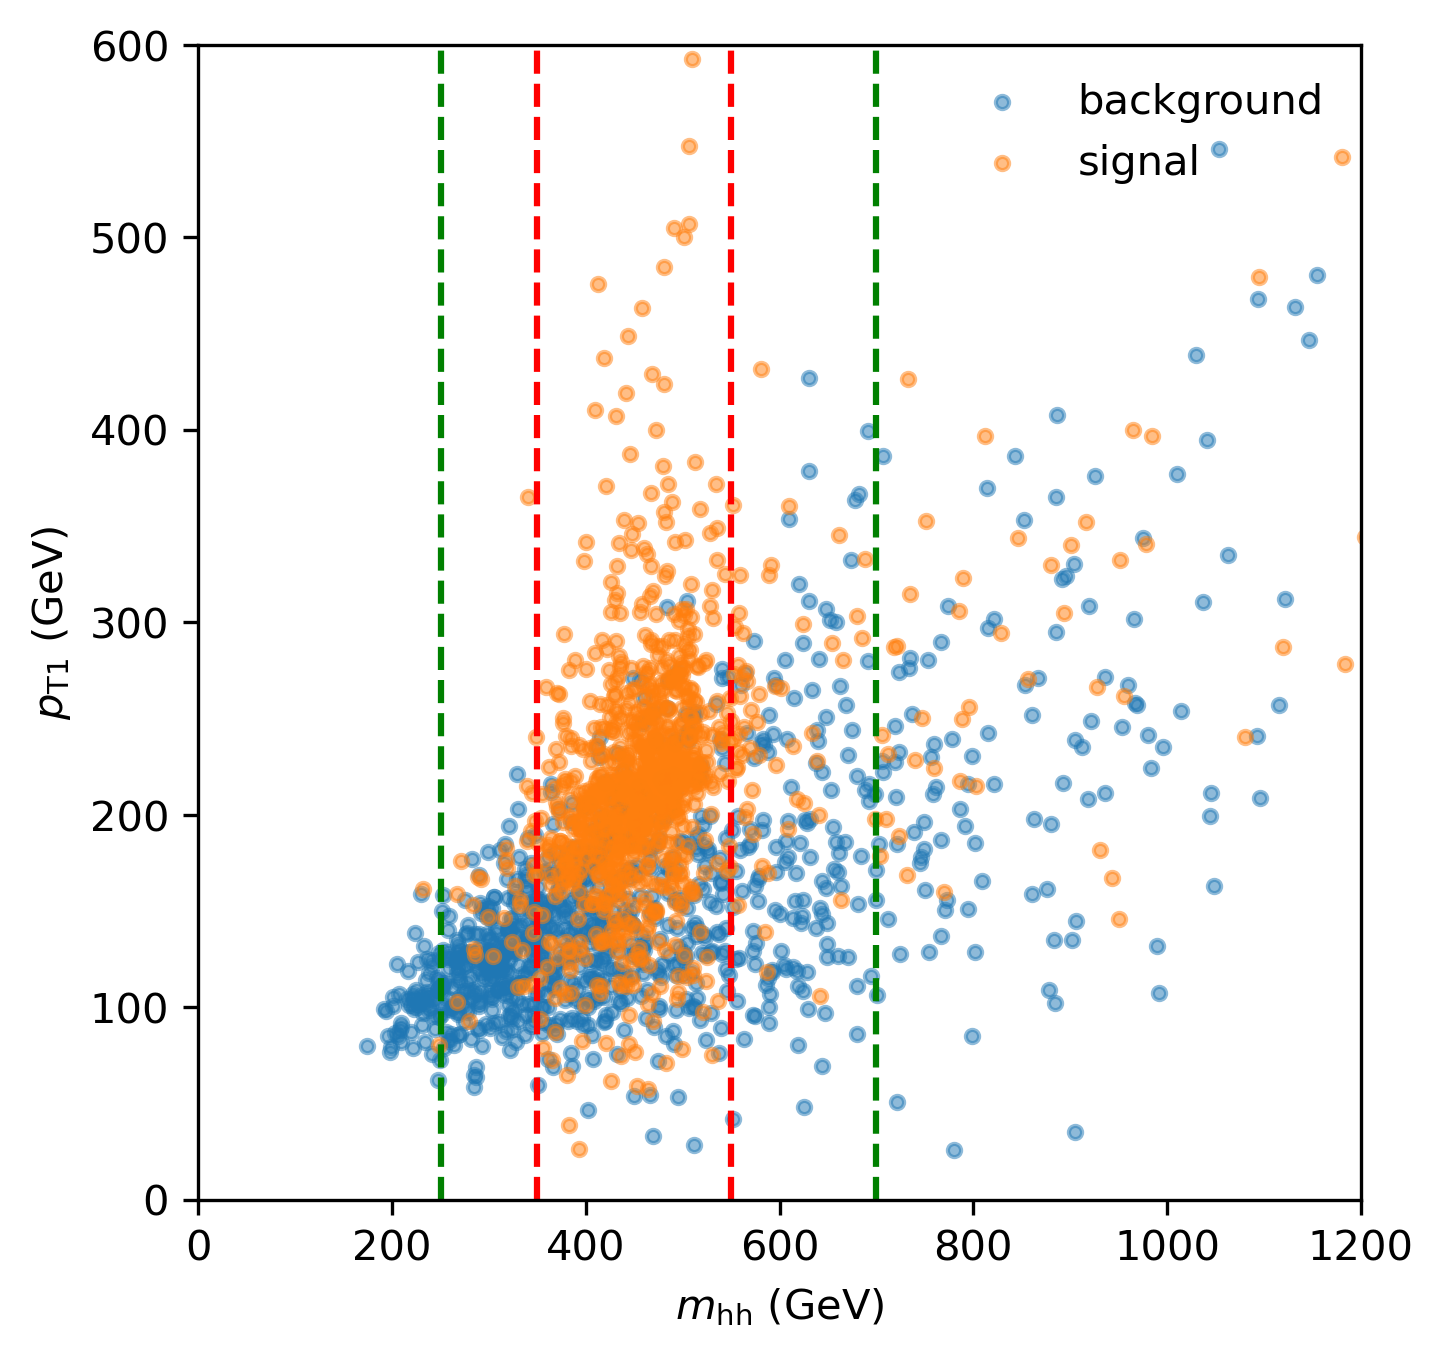
\includegraphics[width=0.45\textwidth]{scatter_plot_mhh_pt1-500GeV.png}
			}
			\subfloat[$m_H = \text{1000 GeV}$]{
				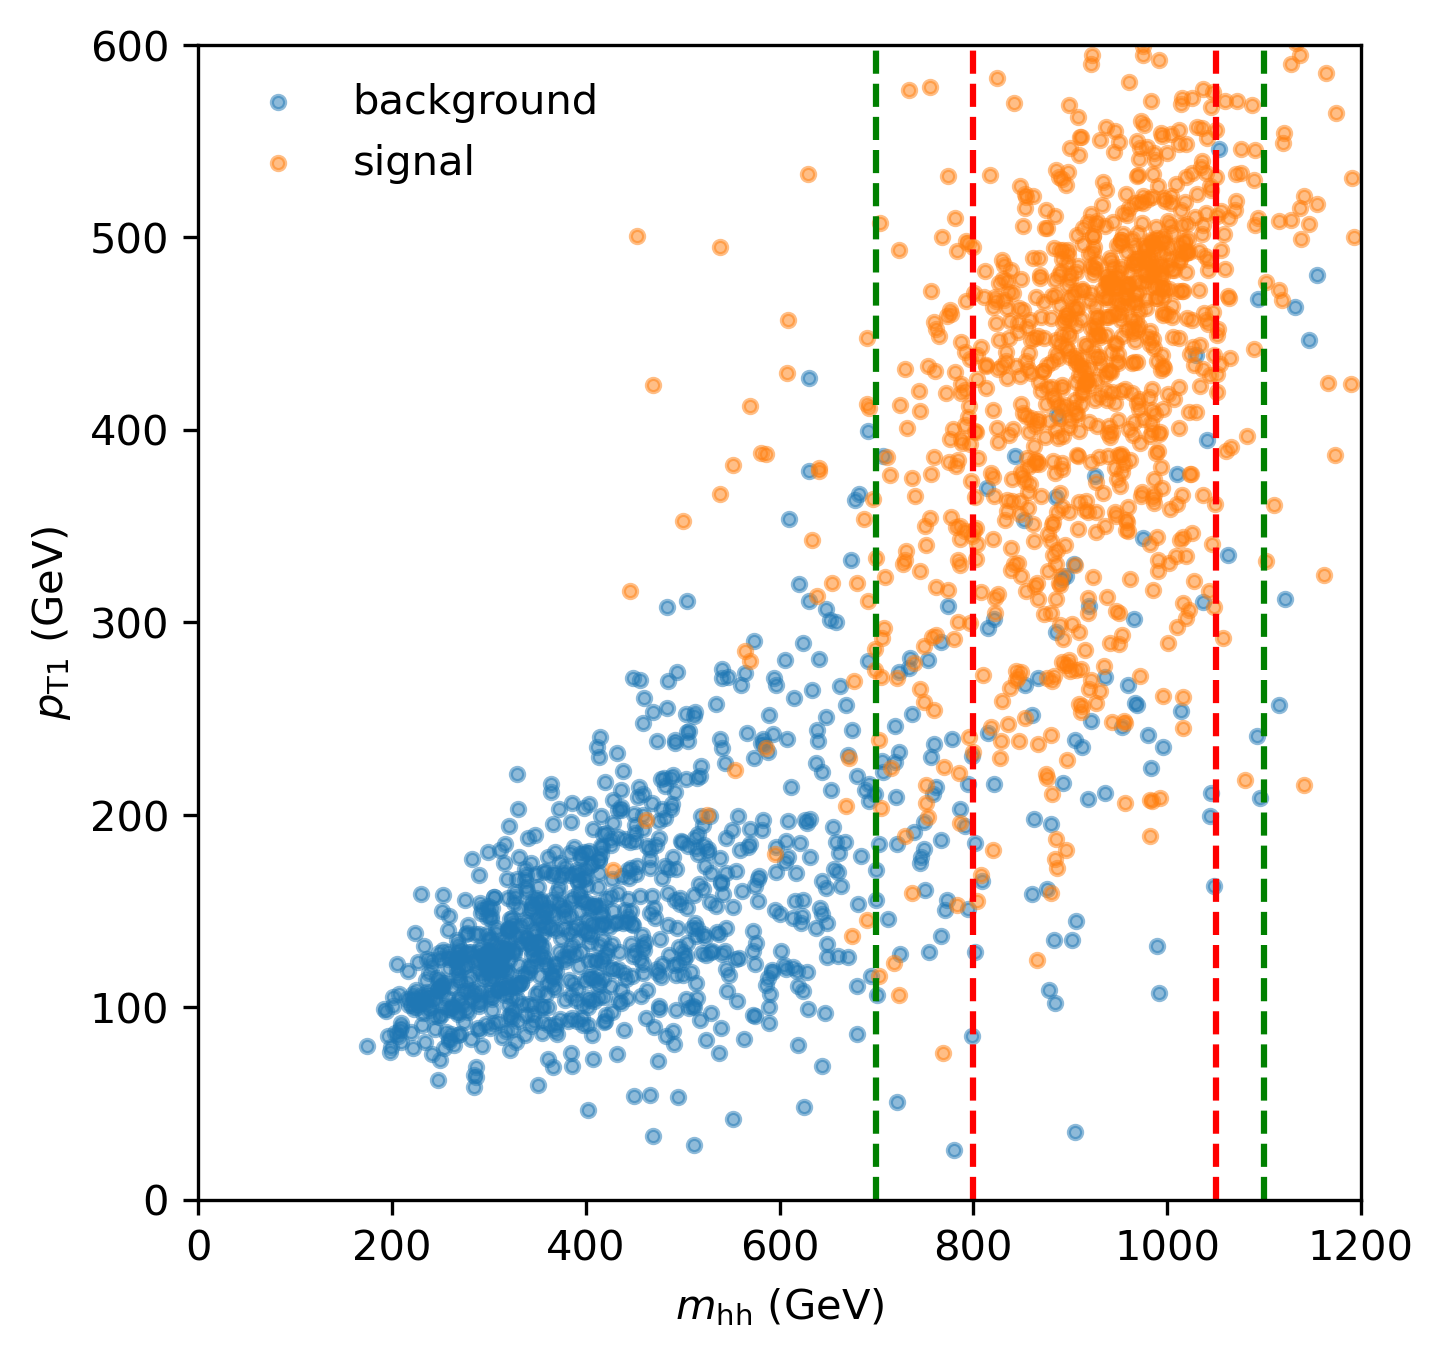
\includegraphics[width=0.45\textwidth]{scatter_plot_mhh_pt1-1000GeV.png}
			}
			\caption{The scatter plots of the transverse momentum of leading Higgs candidate $p_{\text{T}1}$ and total invariant mass $m_{hh}$ distribution. The signal region is between the red dashed lines. The sideband region is between the green dashed lines and excludes the signal region.}
			\label{fig:pt1_mhh_scatter_plot}
		\end{figure}
	% subsection correlation_matrix (end)	
% section cwola_hunting (end)		
\section{Physical data augmentation}% (fold)
\label{sec:physical_data_augmentation}
	The physical augmentations are inspired by Reference~\cite{Dillon:2023zac}, which considers the rotation and smearing augmentations. These augmentations reflect both the symmetries in the physical event and the experimental resolution of the detector.
	\subsection{Original training data}% (fold)
	\label{sub:original_training_data}
		The signal is the resonant Higgs boson pairs production in the four-$b$ quarks channel. In this section, the Higgs boson pair is produced by the heavy CP-even scalar $H$ with mass $m_H = \text{500 GeV}$. The background consists of QCD multi-jet events. The basic requirement is the ``four-tag cut,'' which requires at least four $b$-tagged $R = 0.4$ anti-$k_t$ jets with $p_\text{T} > \text{40 GeV}$ and $\abs{\eta} < 2.5$. Only the events passing the four-tag cut are used in the following analysis.
		
		The training samples consist of 50k signal events and 50k background events and the testing samples consist of 5k signal events and 5k background events.

		The Higgs candidates are reconstructed by the $\text{min-}\Delta R$ pairing method. The input features are similar to the previous case (Table~\ref{tab:DNN_variables}), but the $b$-tagging information is excluded.
	% subsection original_training_data (end)
	\subsection{Physical augmentation}% (fold)
	\label{sub:physical_augmentation}
		We consider three different physical augmentations.

		\begin{enumerate}
			\item Azimuthal rotation: The whole final state is rotated by an angle $\phi$ randomly sampled from $[0, 2\pi]$.
			\item $\eta-\phi$ smearing: The $\left( \eta,\phi \right) $ coordinate of Higgs candidates are resampled according to a Normal distribution centered on the original coordinate and with a standard deviation inversely proportional to the $p_{\text{T}}$
				\begin{equation}
					\eta' \sim \mathcal{N}\left(\eta, \frac{\Lambda}{p_{\text{T}}}\right), \quad \phi' \sim \mathcal{N}\left(\phi, \frac{\Lambda}{p_{\text{T}}}\right)
				\end{equation}
				where $\eta', \phi'$ are the augmented coordinate, $p_{\text{T}}$ is the transverse momentum of the Higgs candidate, and the smearing scale is set to be $\Lambda = \text{10 GeV}$.
			\item $p_\text{T}$ smearing: The $p_{\text{T}}$ of Higgs candidates are resampled according to
				\begin{equation}
					p_{\text{T}}' \sim \mathcal{N}\left( p_{\text{T}}, f(p_{\text{T}}) \right), \quad f(p_{\text{T}}) = \sqrt{0.052 p_{\text{T}}^2 + 1.502p_{\text{T}}}
				\end{equation}
				where $p_{\text{T}}'$ is the augmented transverse momentum, $f\left( p_\text{T} \right) $ is the energy smearing applied by \verb|Delphes| (the $p_{\text{T}}$'s are normalised by $\text{1 GeV}$).
		\end{enumerate}

		Figure~\ref{fig:eta_phi_smearing_eta_distribution}, \ref{fig:eta_phi_smearing_phi_distribution} and \ref{fig:pt_smearing_pt_distribution} are the distributions before and after the augmentation. For the $\eta-\phi$ smearing, the distributions are similar for both cases. For $p_\text{T}$ smearing, it makes the peak broaden and the transverse momentum distribution looks smoother.
		\begin{figure}[htpb]
			\centering
			\subfloat[Leading Higgs]{
				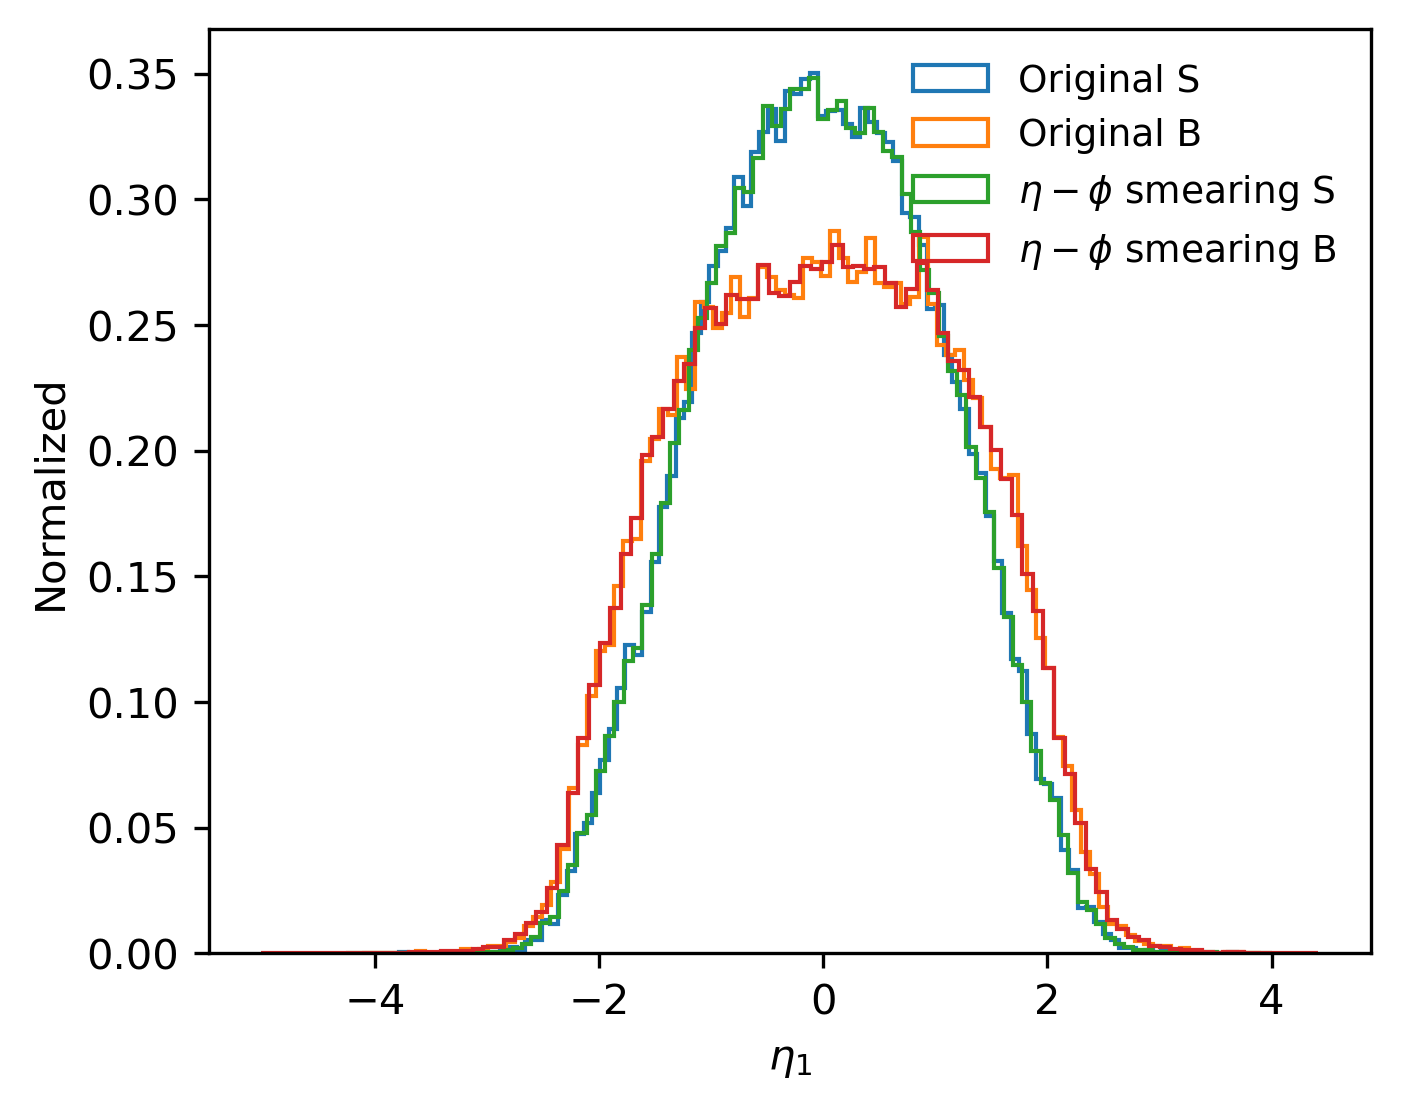
\includegraphics[width=0.45\textwidth]{eta1_distribution_eta_phi_smearing.png}
			}
			\subfloat[Sub-leading Higgs]{
				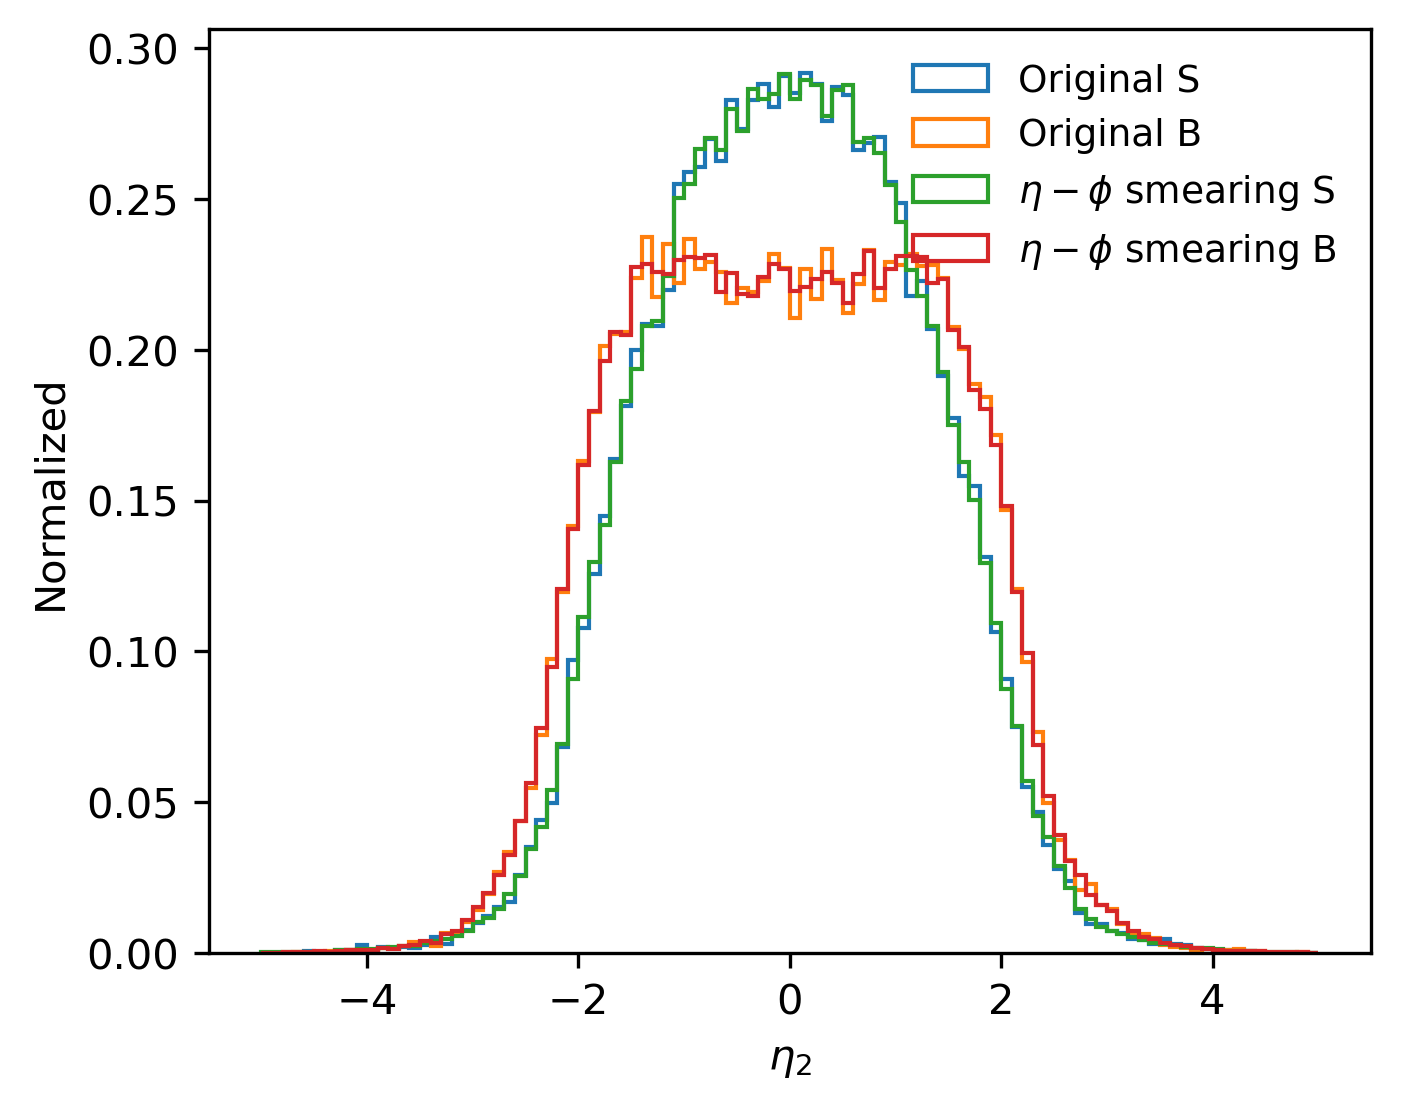
\includegraphics[width=0.45\textwidth]{eta2_distribution_eta_phi_smearing.png}
			}
			\caption{The pseudorapidity distribution before and after the $\eta-\phi$ smearing augmentation. $\eta_1$ and $\eta_2$ are the pseudorapidities of the leading and the sub-leading Higgs candidate, respectively.}
			\label{fig:eta_phi_smearing_eta_distribution}
		\end{figure}
		\begin{figure}[htpb]
			\centering
			\subfloat[Leading Higgs]{
				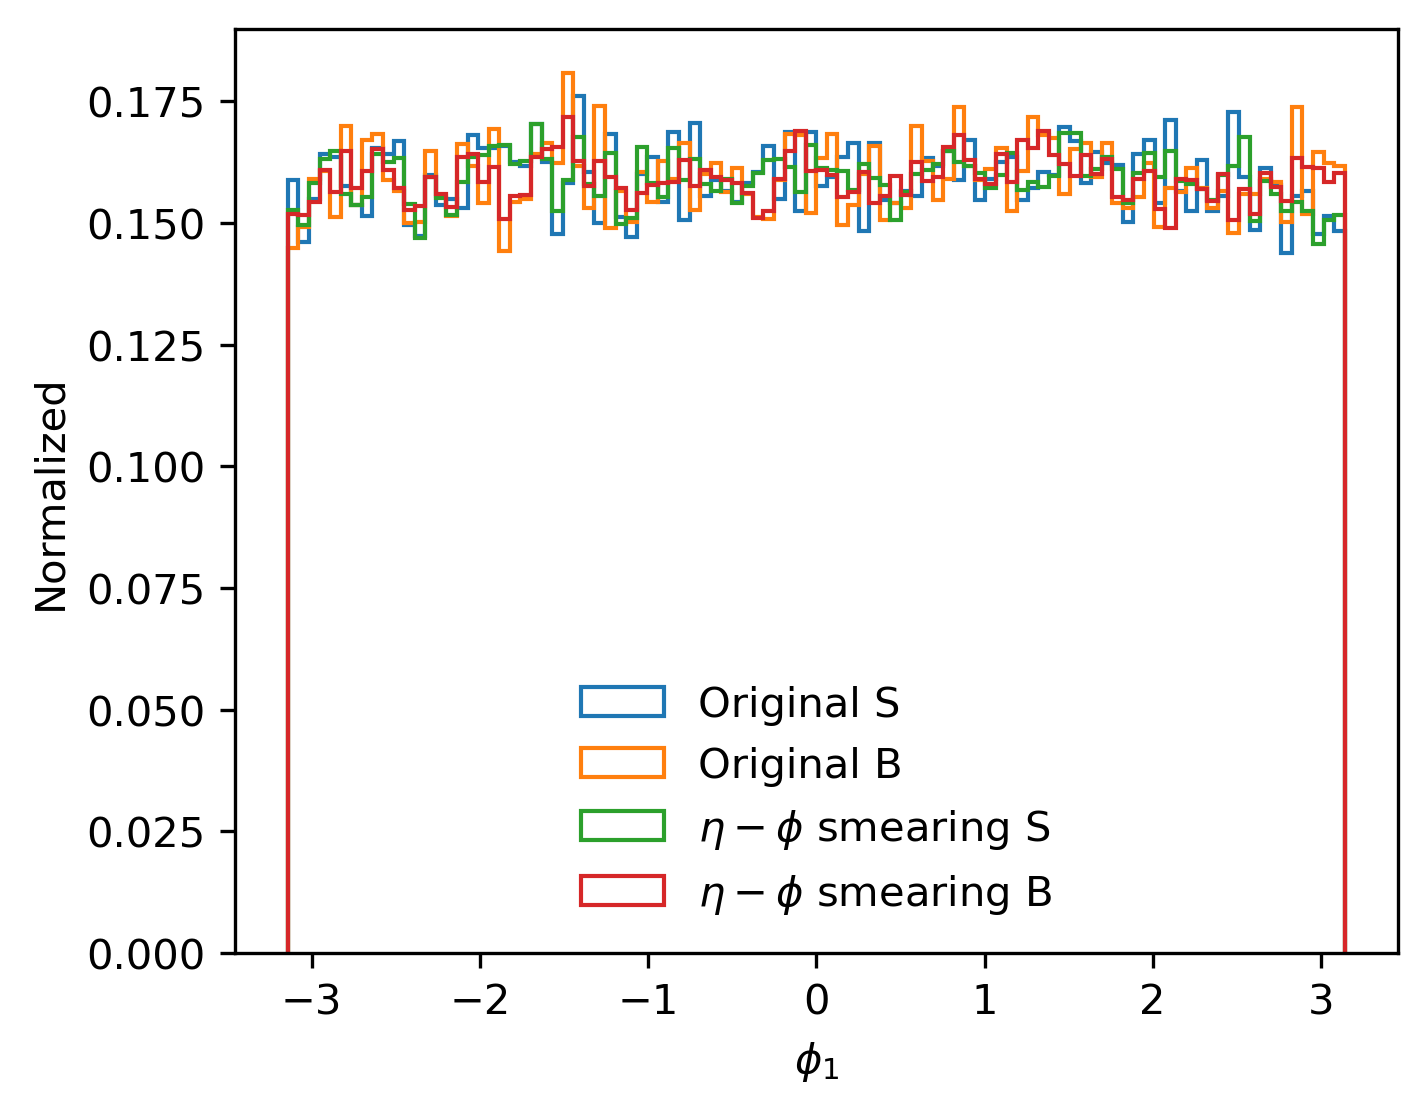
\includegraphics[width=0.45\textwidth]{phi1_distribution_eta_phi_smearing.png}
			}
			\subfloat[Sub-leading Higgs]{
				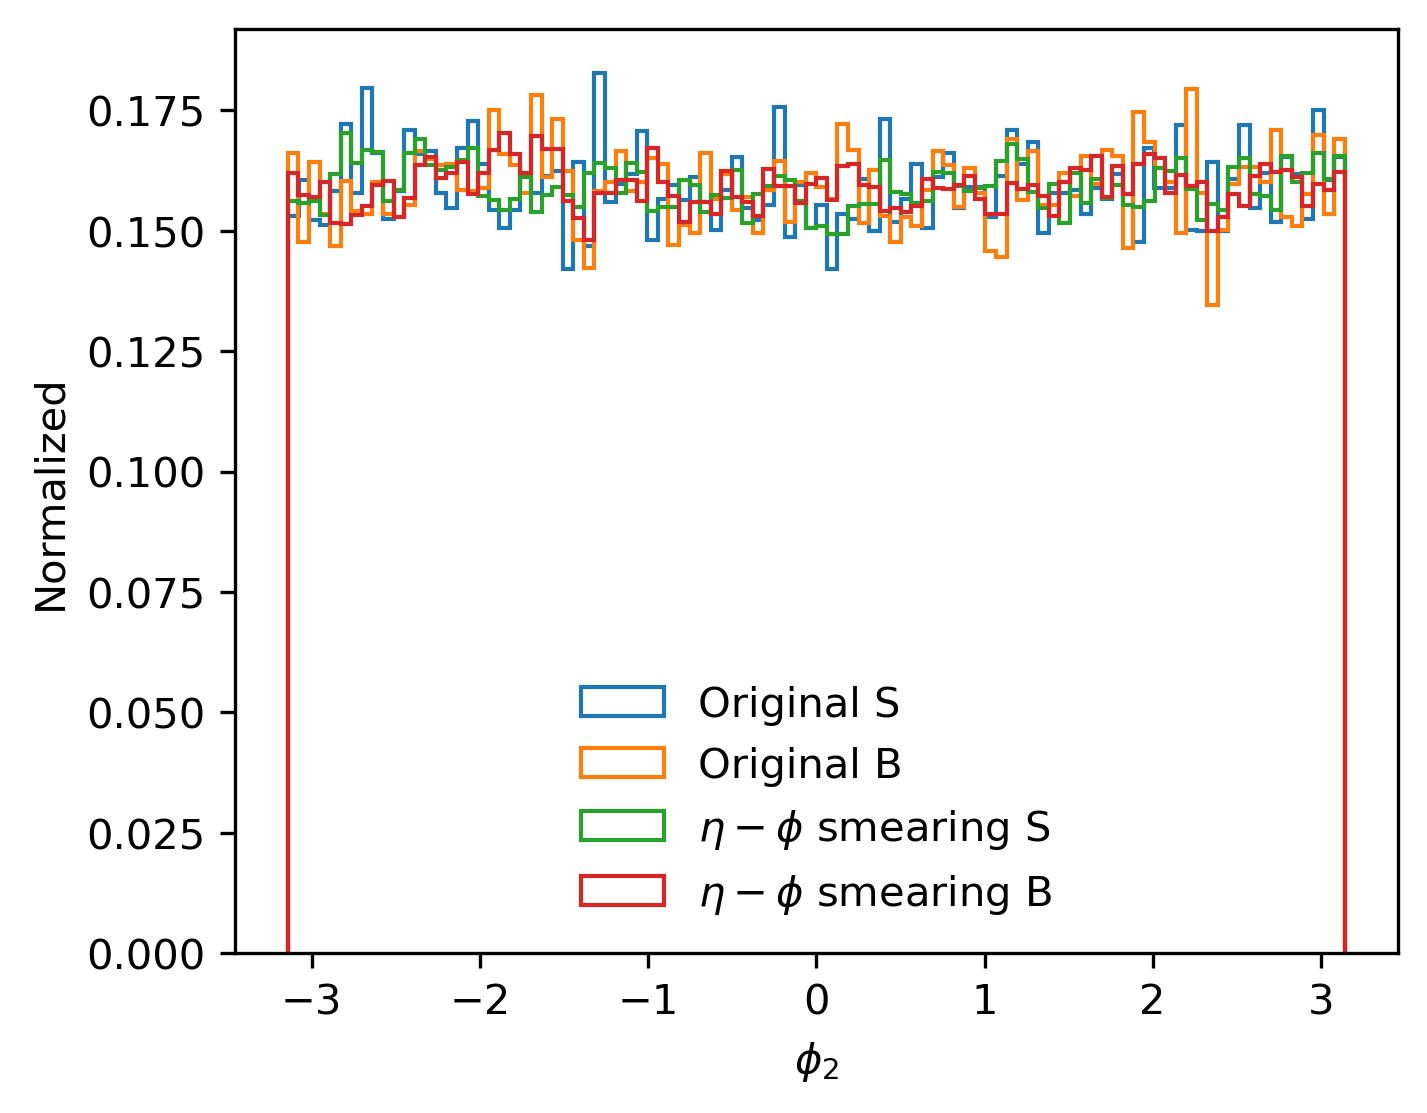
\includegraphics[width=0.45\textwidth]{phi2_distribution_eta_phi_smearing.png}
			}
			\caption{The azimuthal angle distribution before and after the $\eta-\phi$ smearing augmentation. $\phi_1$ and $\phi_2$ are the azimuthal angles of the leading and the sub-leading Higgs candidate, respectively.}
			\label{fig:eta_phi_smearing_phi_distribution}
		\end{figure}
		\begin{figure}[htpb]
			\centering
			\subfloat[Leading Higgs]{
				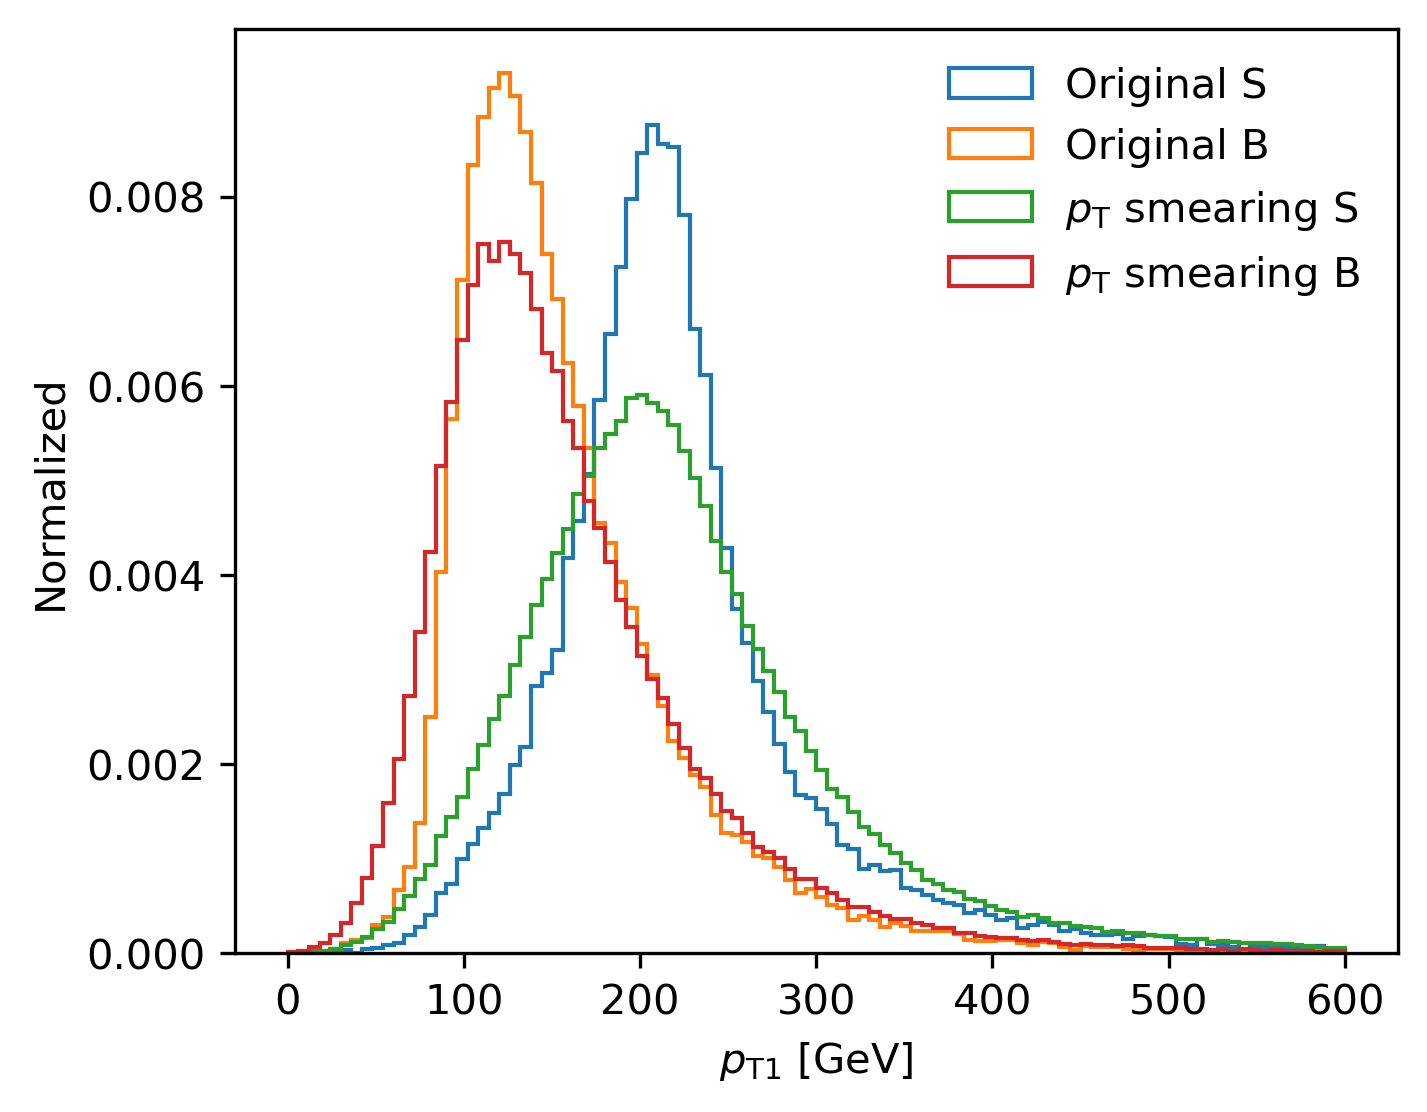
\includegraphics[width=0.45\textwidth]{pt1_distribution_pt_smearing.png}
			}
			\subfloat[Sub-leading Higgs]{
				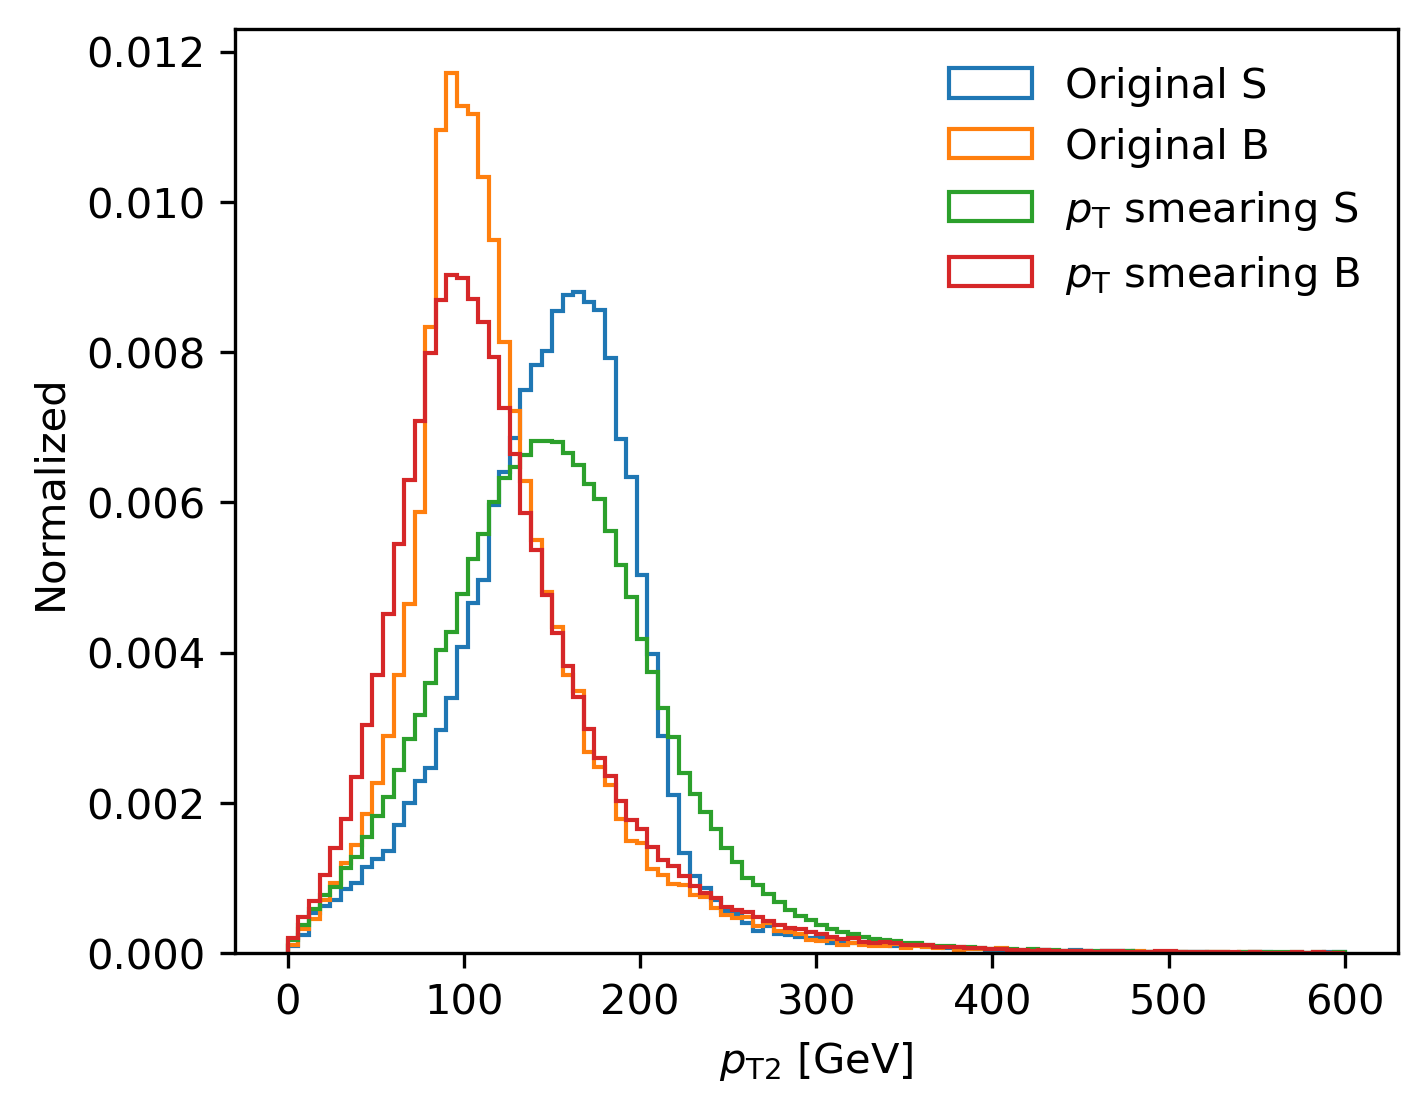
\includegraphics[width=0.45\textwidth]{pt2_distribution_pt_smearing.png}
			}
			\caption{The transverse momentum distribution before and after the $p_{\text{T}}$ smearing augmentation. $p_{\text{T1}}$ and $p_{\text{T2}}$ are the transverse momentum of the leading and the sub-leading Higgs candidates, respectively.}
			\label{fig:pt_smearing_pt_distribution}
		\end{figure}

		For each type of augmentation, we test ``$n$ times augmentation'' with different $n$. The $n$ times augmentation means for one original sample, we generate $n$ augmented samples. Additionally, we test another case that applies all augmentations at the same time.
	% subsection physical_augmentation (end)
	\subsection{Training results}% (fold)
	\label{sub:training_results_physical_augmentation}
	
		Table~\ref{tab:original_sample_training_results} presents the DNN classification training results of the original sample. Table~\ref{tab:augmentation_sample_training_results} are the training results of the augmented samples. For each type of augmentation, they all can improve the ACC by about 4\%. The differences among the various augmentation are not significant. The 10-times augmentation has the best results, but the difference between the 5-times and 10-times augmentation is very small. It seems that the performance of this classifier is saturated.
		\begin{table}[htpb]
			\centering
			\caption{The training results of original samples. ACC is the best accuracy and AUC is the area under the ROC curve. The average and standard deviation of 10 training are presented.}
			\label{tab:original_sample_training_results}
			\begin{tabular}{c|c}
			    & Original \\ \hline
			ACC & $0.845 \pm 0.015$    \\
			AUC & $0.917 \pm 0.005$    
			\end{tabular}
		\end{table}
		\begin{table}[htpb]
			\centering
			\caption{The training results of augmented samples. ACC is the best accuracy and AUC is the area under the ROC curve. The average and standard deviation of 10 training are presented.}
			\label{tab:augmentation_sample_training_results}
			\begin{tabular}{l|c|cccc}
									  &     & Rotation          & $\eta-\phi$ smear & $p_{\text{T}}$ smear & All               \\ \hline
			\multirow{2}{*}{3 times}  & ACC & $0.880 \pm 0.007$ & $0.879 \pm 0.010$ & $0.882 \pm 0.003$    & $0.875 \pm 0.011$ \\
									  & AUC & $0.950 \pm 0.007$ & $0.949 \pm 0.008$ & $0.951 \pm 0.003$    & $0.942 \pm 0.012$ \\ \hline
			\multirow{2}{*}{5 times}  & ACC & $0.887 \pm 0.002$ & $0.887 \pm 0.001$ & $0.890 \pm 0.002$    & $0.889 \pm 0.003$ \\
									  & AUC & $0.955 \pm 0.001$ & $0.955 \pm 0.001$ & $0.957 \pm 0.001$    & $0.956 \pm 0.001$ \\ \hline
			\multirow{2}{*}{10 times} & ACC & $0.889 \pm 0.001$ & $0.889 \pm 0.002$ & $0.892 \pm 0.002$    & $0.892 \pm 0.002$ \\
									  & AUC & $0.956 \pm 0.001$ & $0.956 \pm 0.001$ & $0.958 \pm 0.001$    & $0.958 \pm 0.000$
			\end{tabular}
		\end{table}	
		
	% subsection training_results_physical_augmentation (end)

% section physical_data_augmentation (end)		
\bibliographystyle{plain}
\bibliography{reference}
		
\end{document} 

